%%******************************************%%
%%                                          %%
%%        Modello di tesi di laurea         %%
%%            di Michele Vaccari            %%
%%                                          %%
%%            28 dicembre 2017              %%
%%                                          %%
%%******************************************%%


% I seguenti commenti speciali impostano:
% 1. PDFLaTeX come motore di composizione;
% 2. tesi.tex come documento principale;
% 3. il controllo ortografico italiano per l'editor.


% !TEX encoding = UTF-8
% !TEX TS-program = pdflatex
% !TEX root = tesi.tex
% !TEX spellcheck = it-IT

\documentclass[
	12pt,		% corpo del font principale
	a4paper,	% carta A4
	twoside,	% impagina per fronte-retro
	openright,	% inizio capitoli a destra
	titlepage	% dopo il titolo ho una nuova pagina
	]{book}

%**************************************************************
% Importazione package
%************************************************************** 

\usepackage[T1]{fontenc}	% codifica dei font:
							% NOTA BENE! richiede una distribuzione *completa* di LaTeX

\usepackage[utf8]{inputenc}	% codifica di input; anche [latin1] va bene
							% NOTA BENE! va accordata con le preferenze dell'editor

\usepackage[english,italian]{babel}	% per scrivere in italiano e in inglese;
									% l'ultima lingua (l'italiano) risulta predefinita

\usepackage{bookmark}	% segnalibri

\usepackage{caption}	% didascalie

\usepackage[norules,signatures]{frontespizio}	% per il frontespizio

\usepackage{graphicx}	% immagini

%\usepackage{url}	% per scrivere gli indirizzi Internet

\usepackage{hyperref}	% collegamenti ipertestuali

\usepackage[dvipsnames]{xcolor}	% colori

\usepackage{emptypage}

\usepackage{listings}

\usepackage[binding=5mm]{layaureo}	% margini ottimizzati per l'A4; rilegatura di 5 mm

\usepackage{lipsum}

\usepackage[autostyle,italian=guillemets]{csquotes}	% gestisce automaticamente i caratteri (")

\usepackage{guit}

\usepackage[backend=biber,style=numeric,hyperref,backref]{biblatex}
						% eccellente pacchetto per la bibliografia;
						% produce uno stile di citazione autore-anno;
						% lo stile "numeric-comp" produce riferimenti numerici
						% per includerlo nel documento bisogna:
						% 1. compilare una prima volta tesi.tex;
						% 2. eseguire: biber tesi
						% 3. compilare ancora tesi.tex.

\usepackage[italian]{varioref}

\usepackage{amsmath}

\usepackage{booktabs}

%**************************************************************
% file contenente le impostazioni della tesi
%**************************************************************

%**************************************************************
% Frontespizio
%**************************************************************
\newcommand{\myName}{Michele Vaccari}											% autore
\newcommand{\myUni}{Università degli Studi di Ferrara}							% università
\newcommand{\myCourse}{Corso di Laurea in Ingegneria Elettronica e Informatica}	% corso di laurea
\newcommand{\myTitle}{Progettazione e Realizzazione di un Sistema Software per il Tracciamento Indoor delle Risorse Umane e Materiali}

%**************************************************************
% Impostazioni di graphicx
%**************************************************************
\graphicspath{{immagini/}}	% cartella dove sono riposte le immagini


%**************************************************************
% Impostazioni di xcolor
%**************************************************************
\definecolor{webgreen}{rgb}{0,.5,0}
\definecolor{webbrown}{rgb}{.6,0,0}


%**************************************************************
% Impostazioni di hyperref
%**************************************************************
\hypersetup{
	%hyperfootnotes=false,
	%pdfpagelabels,
	%draft,	% = elimina tutti i link (utile per stampe in bianco e nero)
	colorlinks=true,
	linktocpage=true,
	pdfstartpage=1,
	pdfstartview=FitV,
	% decommenta la riga seguente per avere link in nero (per esempio per la stampa in bianco e nero)
	%colorlinks=false, linktocpage=false, pdfborder={0 0 0}, pdfstartpage=1, pdfstartview=FitV,
	breaklinks=true,
	pdfpagemode=UseNone,
	pageanchor=true,
	pdfpagemode=UseOutlines,
	plainpages=false,
	bookmarksnumbered,
	bookmarksopen=true,
	bookmarksopenlevel=1,
	hypertexnames=true,
	pdfhighlight=/O,
	%nesting=true,
	%frenchlinks,
	urlcolor=webbrown,
	linkcolor=RoyalBlue,
	citecolor=webgreen,
	%pagecolor=RoyalBlue,
	%urlcolor=Black, linkcolor=Black, citecolor=Black, %pagecolor=Black,
	pdftitle={\myTitle},
	pdfauthor={\textcopyright\ \myName, \myUni, \myCourse},
	pdfsubject={},
	pdfkeywords={},
	pdfcreator={pdfLaTeX},
	pdfproducer={LaTeX}
}


%**************************************************************
% Impostazioni di biblatex
%**************************************************************
\bibliography{bibliografia}	% database di biblatex

\defbibheading{bibliography}
{
	%\cleardoublepage
	%\clearpage
	\phantomsection
	%\addcontentsline{toc}{chapter}{\bibname}
	\addcontentsline{toc}{chapter}{Bibliografia}
	\chapter*{\bibname\markboth{BIBLIOGRAFIA}{BIBLIOGRAFIA}}
}

\setlength\bibitemsep{1.5\itemsep}	% spazio tra entry

\DeclareBibliographyCategory{web}

\defbibheading{web}{\section*{Siti Web di riferimento}}

%**************************************************************
% Impostazioni di caption
%**************************************************************
\captionsetup{
	%    tableposition=top,
	figureposition=bottom,
	font=small,
	format=hang,
	labelfont=bf
}

%**************************************************************
% Impostazioni di listings
%**************************************************************
% Imposta lo spazio nella list of listing in modo simile alla list of figures/tables
\makeatletter
\let\my@chapter\@chapter
\renewcommand*{\@chapter}{%
  \addtocontents{lol}{\protect\addvspace{10pt}}%
  \my@chapter}
\makeatother


\definecolor{codegreen}{rgb}{0,0.6,0}
\definecolor{codegray}{rgb}{0.5,0.5,0.5}
\definecolor{backcolor}{rgb}{0.98,0.98,0.98}

\renewcommand{\lstlistingname}{Codice}% Listing -> codice
\renewcommand{\lstlistlistingname}{Elenco dei frammenti di codice}% List of Listings -> Frammenti di codice

\lstdefinestyle{mystyle}{
    backgroundcolor=\color{backcolor},   
    commentstyle=\color{Peach}\ttfamily,
    keywordstyle=\color{RoyalBlue},
    numberstyle=\tiny\color{codegray},
    stringstyle=\color{SeaGreen}\ttfamily,
    basicstyle=\footnotesize\ttfamily,
    breakatwhitespace=false,         
    breaklines=true,                 
    captionpos=b,                    
    keepspaces=true,                 
    numbers=left,                    
    numbersep=5pt,                  
    showspaces=false,                
    showstringspaces=false,
    showtabs=false,                  
    tabsize=2,
    frame=trbl, % draw a frame at the top, right, left and bottom of the listing
	frameround=ftff, % angolo in basso a destro curvo
	framesep=4pt, % quarter circle size of the round corners,
	inputencoding=utf8,
    extendedchars=true,
    literate={á}{{\'a}}1 {à}{{\`a}}1 {é}{{\'e}}1 {è}{{\`e}}1 {ù}{{\`u}}1 {ò}{{\`o}}1,
    belowskip=1em,
    aboveskip=1em,
}

 
\lstset{style=mystyle}

\lstdefinelanguage{JavaScript}
{
  % list of keywords
  morekeywords={ true, false, catch, function, break, new, class, extends, var, require, switch, return, import, if, else, while, for, this, View, Text, StyleSheet},
  sensitive=false, % keywords are not case-sensitive
  morecomment=[l]{//}, % l is for line comment
  morecomment=[s]{/*}{*/}, % s is for start and end delimiter
  morestring=[b]" % defines that strings are enclosed in double quotes
}

\lstdefinelanguage{JSON}
{
  % list of keywords
  morekeywords={string, boolean, int, Array, Node, Asset, AssetDetail, Filter, FilterItem},
  sensitive=false, % keywords are not case-sensitive
  morecomment=[l]{//}, % l is for line comment
  morecomment=[s]{/*}{*/}, % s is for start and end delimiter
  morestring=[b]" % defines that strings are enclosed in double quotes
}	% file con le impostazioni personali

\begin{document}
	%\pagestyle{plain}
	% !TEX encoding = UTF-8
% !TEX TS-program = pdflatex
% !TEX root = ../tesi.tex
% !TEX spellcheck = it-IT

%**************************************************************
% Frontespizio 
%**************************************************************
\begin{frontespizio}
	
	\NCandidato{Tesi di Laurea di}
	\Margini{2cm}{2.4cm}{2cm}{2.4cm}
	
	\Preambolo{\renewcommand{\frontlogosep}{1.4cm}}
	
	\Preambolo{\renewcommand{\frontinstitutionfont}{\fontsize{18}{17}\bfseries}}
	\Preambolo{\renewcommand{\frontdivisionfont}{\fontsize{14}{16}\selectfont}}
	\Preambolo{\renewcommand{\fronttitlefont}{\fontsize{22}{32}\bfseries\vspace{1.5cm}}}
	
	\Preambolo{\renewcommand{\frontfixednamesfont}{\fontsize{12}{14}\selectfont}}
	\Preambolo{\renewcommand{\frontnamesfont }{\fontsize{14}{21}\selectfont\vspace{1.8cm}}}
	
	\Preambolo{\renewcommand{\frontadjustforsignatures}{1cm}}
	
	\Istituzione{UNIVERSIT\`A DEGLI STUDI DI FERRARA}
	\Logo[5.5cm]{immagini/logo-unife}
	
	\Divisione{\mbox{}}
	
	\Corso[Laurea]{Ingegneria Elettronica e Informatica}
	\Titolo{Progettazione e Realizzazione di un Sistema \\ Software per il Tracciamento Indoor \\ delle Risorse Umane e Materiali}
	\Candidato[]{Michele Vaccari}
	\Relatore{Ing. Mauro Tortonesi}
	\Annoaccademico{2016 -- 2017}
	
\end{frontespizio}	% frontespizio
	%**************************************************************
	% Materiale iniziale
	%**************************************************************
	\frontmatter
	% !TEX encoding = UTF-8
% !TEX TS-program = pdflatex
% !TEX root = ../tesi.tex
% !TEX spellcheck = it-IT

%**************************************************************
% Ringraziamenti
%**************************************************************
\cleardoublepage
\pdfbookmark{Ringraziamenti}{ringraziamenti}


\begingroup
\let\clearpage\relax
\let\cleardoublepage\relax
\let\cleardoublepage\relax
\chapter*{Ringraziamenti}

In primo luogo vorrei ringraziare l'Ing. Mauro Tortonesi, per l’aiuto e il sostegno fornitomi durante la stesura del lavoro.\\


Un ringraziamento speciale va a Giovanni Borghi, a Sabrina Formica e in generale a tutto il team di Evomatic s.r.l., per avermi permesso di svolgere il lavoro di tirocinio in un ambiente sereno e informale. Un ringraziamento di dovere va anche a Lorenzo Visentin, mio tutor aziendale, per avermi seguito amichevolmente e per avermi dato i consigli e i suggerimenti necessari per lo sviluppo del progetto formativo.\\


Ringrazio di cuore la mia famiglia, che mi ha sostenuto sia moralmente che economicamente durante questo percorso di studi universitario, e Arianna che mi ha sempre accompagnato anche nei momenti di totale abbandono, senza mai pretendere troppo da me, sostenendomi sempre.\\


Infine, ringrazio tutti gli amici e compagni di corso per essermi stati vicini in ogni momento, per ogni aiuto e supporto durante il mio percorso universitario.\\

\bigskip

\noindent Ferrara, Febbraio 2018
\hfill Michele Vaccari

\endgroup	% ringraziamenti
	% !TEX encoding = UTF-8
% !TEX TS-program = pdflatex
% !TEX root = ../tesi.tex
% !TEX spellcheck = it-IT

%**************************************************************
% Indici
%**************************************************************
\cleardoublepage
\pdfbookmark{\contentsname}{tableofcontents}
\setcounter{tocdepth}{2}
\markboth{\contentsname}{\contentsname}

\tableofcontents	% indice generale

\clearpage

%\begingroup
%	
%	\let\newpage\relax
%	\let\clearpage\relax
%	\let\cleardoublepage\relax
%	
%	%*******************************************************
%	% Elenco delle figure
%	%*******************************************************
%	\pdfbookmark{\listfigurename}{lof}
%	\listoffigures		% elenco delle figure
%	
%	%*******************************************************
%	% Elenco delle tabelle
%	%*******************************************************
%	\pdfbookmark{\listtablename}{lot}
%	\listoftables		% elenco delle tabelle
%	
%	%*******************************************************
%	% Elenco delle porzioni di codice
%	%*******************************************************
%	\pdfbookmark{\listtablename}{loc}
%	\lstlistoflistings
%
%\endgroup			% indici
	
	%**************************************************************
	% Materiale principale
	%**************************************************************
	\mainmatter
	% !TEX encoding = UTF-8
% !TEX TS-program = pdflatex
% !TEX root = ../tesi.tex
% !TEX spellcheck = it-IT

%**************************************************************
% Introduzione
%**************************************************************
\cleardoublepage
\pdfbookmark{Introduzione}{introduzione}

\chapter*{Introduzione}
\addcontentsline{toc}{chapter}{Introduzione}
\markboth{\MakeUppercase{Introduzione}}{\MakeUppercase{Introduzione}}

Il tracciamento di una risorsa, ovverosia la possibilità di conoscerne la posizione geografica e di tracciarne gli spostamenti in tempo reale, è una necessità che si sta affermando prepotentemente nel mondo odierno. Molte delle applicazioni che si trovano in uno smarthphone sfruttano, volontariamente o meno, la posizione del dispositivo per migliorare i servizi offerti dai vari applicativi.

Nella maggioranza dei dispositivi è presente un ricevitore GPS che consente di localizzare, tramite segnale satellitare, un terminale in uno spazio aperto. Tuttavia questa tecnologia non è disponibile quando si è all'interno di uno spazio chiuso in cui non è possibile utilizzare il segnale satellitare, che risulterebbe troppo attenuato per fornire indicazioni di posizionamento precise. In questo caso, è necessario adottare tecnologie di localizzazione espressamente pensate per ambienti indoor.

La società Evomatic s.r.l., nello sviluppo della propria piattaforma per la gestione delle risorse in movimento, utilizza in modo massivo la tecnologia GPS per consentire la geolocalizzazione delle risorse dei propri clienti in campo aperto. L'interesse della società è quello di estendere i servizi offerti dalla piattaforma anche in ambito indoor, con il riutilizzo della maggior parte delle tecnologie impiegate per lo sviluppo dei servizi di localizzazione in campo aperto, quali l'uso di TAG Bluetooth Low Energy (BLE) e di smartphone con sistema Android.

Questa tesi descrive la realizzazione di un sistema software per la localizzazione indoor offrendo una soluzione che fa uso di tecnologia BLE presente all'interno di molti smartphone Android disponibili in commercio. Le attività di progettazione e sviluppo del sistema sono state svolte durante il tirocinio presso la divisione sistemi di localizzazione satellitare e Internet-of-Things di Evomatic s.r.l., che si occupa della gestione e della manutenzione dei servizi in produzione nella propria piattaforma e, inoltre, svolge le attività di ricerca e sviluppo per l’integrazione di nuove funzionalità fruibili dai vari clienti nella piattaforma stessa.

Il sistema sviluppato è composto da vari componenti che cooperano per fornire la posizione di una risorsa in tempo reale. Dal browser si accede all'applicazione web che consente di caricare una piantina dell'ambiente in cui si desiderano monitorare le risorse. Dall'applicazione web, inoltre, è possibile gestire il posizionamento, la modifica della posizione e l'eliminazione dei TAG BLE, che operano come beacon, all'interno della piantina caricata precedentemente. Si posizionano i TAG BLE all'interno dell'ambiente indoor coerentemente con quanto fatto nell'applicazione web. Si avvia l'applicazione installata nello smartphone Android che permette di avviare la rilevazione della risorsa, previa autenticazione. L'applicazione Android, invia periodicamente i dati che ha raccolto dai beacon BLE per effettuare il calcolo della posizione e, se ci sono problemi di connessione, i dati vengono inviati appena è possibile stabilire una connessione. Da quel momento è possibile visualizzare dall'applicazione web l'ultima posizione valida della risorsa all'interno della piantina con informazioni riguardo il nome della risorsa, l'orario e la data della rilevazione.

Il sistema progettato è realizzato in Java per quanto riguarda lo sviluppo dell'applicazione Android, mentre per lo sviluppo degli altri componenti si è utilizzato in modo predominante il linguaggio Javascript. Il formato comune utilizzato per l'interscambio dei dati tra i vari componenti è JSON. Per l'interscambio dei dati si sono utilizzati i protocolli MQTT e HTTP. Per le interrogazioni al database interno del sistema Android si è utilizzato il linguaggio SQL specifico per SQLite, mentre per le interrogazioni al database di Microsoft SQL Server si è utilizzato il linguaggio SQL proprietario di Microsoft.

Il funzionamento e l'efficienza del sistema progettato sono stati verificati attraverso una serie di test effettuati all'interno degli uffici della società Evomatic s.r.l.. Inizialmente si è verificato il corretto funzionamento del sistema per il rilevamento real time della posizione di una singola risorsa in una singola stanza, successivamente si è esteso il test per il rilevamento della posizione di una singola risorsa in più stanze per poi estendere il numero di risorse.

La tesi è organizzata secondo la seguente struttura: il Capitolo~\ref{cap:localizzazione-indoor} introduce la geolocalizzazione indoor e la differenza con la geolocalizzazione in campo aperto; il Capitolo~\ref{cap:localizzazione-con-rssi} introduce l'RSSI e il suo utilizzo nell'algoritmo di trilaterazione per il calcolo della posizione; il Capitolo~\ref{cap:progetto} presenta i vincoli di progetto e l'architettura del sistema; il Capitolo~\ref{cap:tecnologie-utilizzate} descrive le tecnologie usate nel sistema; il Capitolo~\ref{cap:implementazione} descrive l'implementazione dei vari componenti del sistema progettato; il Capitolo~\ref{cap:risultati-sperimentali} riporta i risultati sperimentali che descrivono le prestazioni del sistema; infine un capitolo conclusivo riporta alcune considerazioni generali sul lavoro svolto e sviluppi futuri.

Durante la progettazione e lo sviluppo del sistema si è cercato di disaccoppiare i diversi componenti in modo da renderli meno sensibili a modifiche e possibili malfunzionamenti.
Nella realizzazione del sistema si è tralasciata la possibilità di visualizzare lo storico delle posizioni di ogni risorsa, concentrandosi nella visualizzazione della posizione in real time.
	% introduzione
	% !TEX encoding = UTF-8
% !TEX TS-program = pdflatex
% !TEX root = ../tesi.tex
% !TEX spellcheck = it-IT

%*************************************************************
\chapter{Localizzazione indoor}
\label{cap:localizzazione-indoor}
%*************************************************************

La posizione di un dispositivo è un dato di centrale importanza che può essere utilizzato per ottimizzare il dispositivo stesso. Le tecnologie che consentono di ottenere la posizione di una risorsa sono diverse nel caso in cui ci troviamo in campo aperto o in campo chiuso.

L’analisi della tecnologia GPS permette di comprendere come si ottiene la posizione di un dispositivo in campo aperto e le problematiche per cui questa tecnica non può essere utilizzata in campi chiusi come gli ambienti indoor.

Per poter localizzare un dispositivo in ambiente indoor è possibile utilizzare altre tecniche basate anch'esse su portanti radio ma che non utilizzano una rete di satelliti in orbita.

\section{Il GPS e l'ambiente indoor}
Il Global Positioning System (GPS) \cite{wiki:gps} è un sistema di navigazione globale basato su satelliti in orbita. La tecnologia GPS consente di ottenere un'informazione precisa circa la posizione e l'orario in cui un determinato ricevitore effettua la richiesta di localizzazione. Questo è possibile grazie a una rete satellitare in funzione a ogni ora del giorno in ogni condizione climatica. La localizzazione tramite GPS, pertanto, è attendibile a patto che il ricevitore riesca a captare il segnale da almeno quattro satelliti distinti.

In un ambiente più complesso, costituito da muri, aree chiuse, come può essere un palazzo o un ospedale, il segnale GPS risente di forti attenuazioni. Per questo motivo la localizzazione mediante segnale satellitare risulta inefficace.

Questo non vuol dire che è impossibile ottenere la posizione di un dispositivo all'interno di un'area indoor ma significa che la tecnologia GPS è una tecnologia sfruttabile in modo efficiente solo in campo aperto.

\section{La localizzazione indoor}
Il mondo della localizzazione indoor si basa sul concetto di sfruttare l'ambiente e le tecnologie presenti, o comunque di facile reperibilità, per avere la possibilità di localizzare una risorsa anche in ambienti interni. In molti casi pratici l'ecosistema utile alla localizzazione viene creato sfruttando combinazioni delle tecnologie dei dispositivi già presenti in ambiente indoor che sfruttano la portante radio, al fine di ottenere il massimo risultato dai benefici derivanti dall'uso di una tecnica, minimizzando i limiti. Questo approccio è favorito dalla larga diffusione di dispositivi che dispongono nativamente di buona parte di queste tecnologie.

È importante osservare che il risultato ottenuto da queste tecniche di localizzazione non fornisce un dato di posizione ``assoluto'', come normalmente restituito da un'interrogazione GPS, ma viene fornita un’informazione di posizione ``relativa'' che deve poi essere interpretata correttamente per far comprendere all'utente dove è localizzato.

Le tecniche attualmente più utilizzate sfruttano tecnologie come: infrarossi (IR), Bluetooth, identificazione a radio frequenza (RFID), ultrasuoni, tecniche di riconoscimento mediante tracciamento ottico e tecniche basate sui segnali wireless (RSS techniques).

In seguito si è scelto di approfondire, rispetto alle altre tecniche, la localizzazione con RSSI, data la maggior reperibilità della tecnologia che consente di sviluppare questa tecnica. L'hardware Bluetooth, infatti, è comunemente integrato in molti dispositivi e smartphone.
			% localizzazione indoor
	% !TEX encoding = UTF-8
% !TEX TS-program = pdflatex
% !TEX root = ../tesi.tex
% !TEX spellcheck = it-IT

%*************************************************************
\chapter{La localizzazione con RSSI}
\label{cap:localizzazione-con-rssi}
%*************************************************************

Una delle tecniche di localizzazione più comuni per la stima della posizione in ambiente indoor è la tecnica \emph{Anchor based}. Nella tecnica Anchor based un sottoinsieme di nodi della rete, chiamati \emph{anchor} o \emph{beacon}, sono a conoscenza della loro posizione, ottenuta grazie al GPS o avendo stabilito un sistema di coordinate predefinite. Gli altri nodi (\emph{target}) usano le informazioni di posizione dai nodi anchor per determinare la propria posizione. Il ranging tra i beacon e gli altri nodi può essere ottenuto con
\begin{itemize}
	
	\item
	interazione diretta (Single-Hop)
	
	\item 
	indirettamente, per mezzo di nodi intermedi (Multi-Hop)
	
\end{itemize}
Per quanto riguarda il processo di localizzazione, questo può essere affrontato usando la tecnica \emph{Range based}. Nella tecnica Range based vengono effettuate una serie di misurazioni per conoscere la distanza tra beacon e target (\emph{ranging}). A questo punto, con l’algoritmo di trilaterazione (vedi paragrafo \ref{par:trilaterazione}) è possibile stimare la posizione dei nodi target.

\section{Ranging: stima della distanza}
\label{par:ranging}
Per stimare la distanza tra beacon e target si è utilizzata una tecnica di tipo range-based dato che è una tra le tecniche più economiche, essendo l'economicità uno dei requisiti fondamentali e maggiormente apprezzabili quando si va a verificare un'applicazione.
Il primo passo da affrontare in un processo di localizzazione di questo tipo è il ranging.
Il ranging tra due nodi è dunque la tecnica utilizzata da questi per determinare la distanza che si separa. Una delle tecniche su cui ci si può basare per la stima della distanza è la valutazione dell'intensità del segnale ricevuto (RSSI).

\section{Received Signal Strenght (RSSI)}
Valutando l'intensità di un segnale ricevuto è possibile stimare la distanza dalla stazione che l'ha trasmesso. Nel caso di dispositivi Bluetooth quello che si va ad utilizzare è un indicatore di potenza, l'RSSI (Received Signal Strenght Indicator), il quale indica una stima della potenza del segnale ricevuto misurato in dBm. Per andare a valutare la distanza dalla quale questo segnale è stato trasmesso si può utilizzare l'equazione di Friis:

\begin{equation}
\label{eq:friis}
P_R=P_T\frac{G_T G_R \lambda^2}{(4\pi)^2 d^n}
\end{equation}

dove:
\begin{itemize}
	
	\item $P_R$ è la potenza del segnale ricevuto in Watt
	
	\item $P_T$ è la potenza del segnale trasmesso in Watt
	
	\item $G_R$ è il guadagno dell'antenna ricevente
	
	\item $G_T$ è il guadagno dell'antenna trasmittente
	
	\item $\lambda$ è la lunghezza d'onda dove $\lambda=c/f$ dove $c$ è la velocità della luce \\ ($299792458\;m/s$) e $f$ è la frequenza
	
	\item $d$ è la distanza in metri
	
	\item $n$ è la costante di propagazione del segnale, detto anche esponente di propagazione, dipende dall'ambiente in cui ci si trova
	
\end{itemize}

Risulta molto utile, dal punto di vista pratico la seguente formula, che ci permette di convertire la potenza da Watt a dBm, dal momento che l’indicatore RSSI è solitamente espresso in dBm.
\begin{equation}
\label{eq:p-dbm}
P[dBm]=10 \cdot log_{10}(P[W] \cdot 10^3)
\end{equation}

Per motivi di semplicità, è possibile combinare assieme la \ref{eq:friis} e la \ref{eq:p-dbm}. Applicando le proprietà dei logaritmi, si ottiene la seguente formula:
\begin{equation}
RSSI=-(10 \cdot n \cdot log_{10}d - A)
\end{equation}

Dove $A$ è la potenza del segnale ricevuto, in dBm, alla distanza di riferimento di un metro e $n$ è la costante di propagazione del segnale.

In figura \ref{fig:andamento-potenza-distanza} è rappresentato l'andamento ideale dell'indicatore RSSI in ambiente aperto ($n=2$, $A=-40dBm$).

A questo punto è conveniente aggiustare la relazione sopra scritta:
\begin{equation}
log_{10}d = \frac{A - RSSI}{10 \cdot n}
\end{equation}

Infine, isolando la distanza:
\begin{equation}
d = 10^{(\frac{A - RSSI}{10 \cdot n})}
\end{equation}

Quest'ultima formula, ci permette quindi di calcolare la distanza tra due nodi conoscendo il valore di RSSI ed i parametri $A$ e $n$.

\begin{figure}[htp]
	\centering
	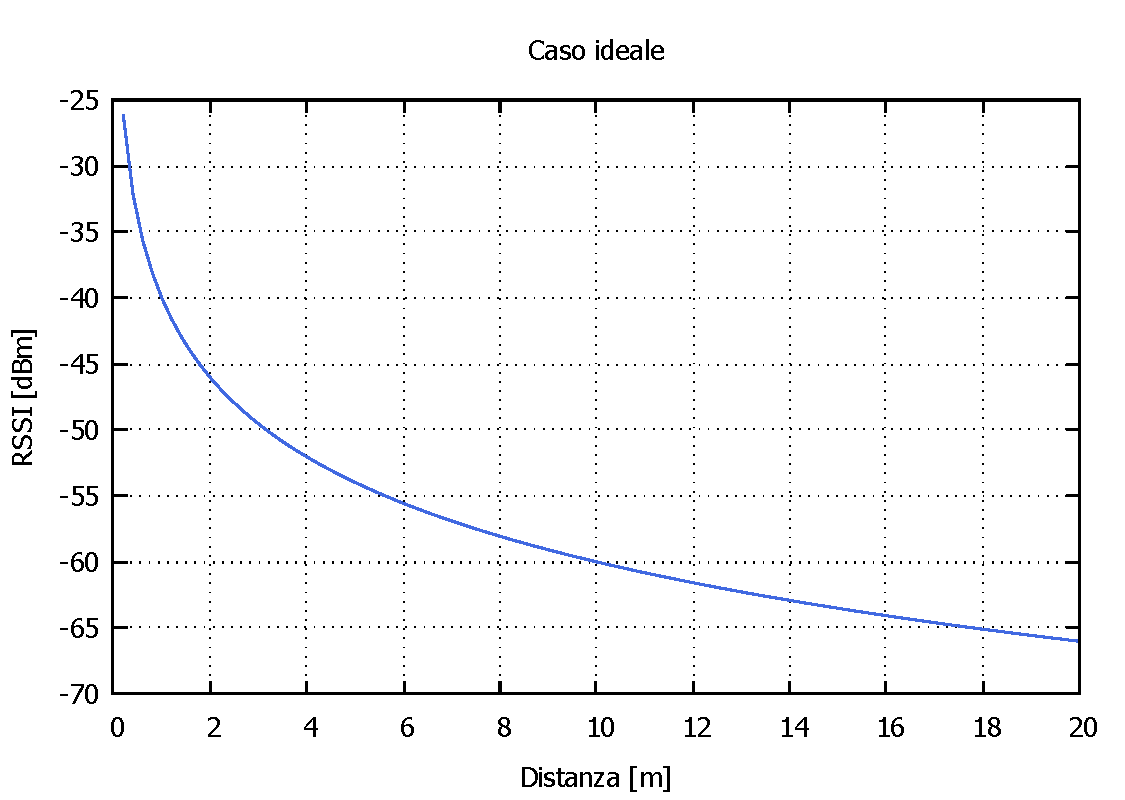
\includegraphics[height=\textheight/3]{andamento-potenza-distanza}
	\caption{Andamento ideale della potenza ricevuta in funzione della distanza}
	\label{fig:andamento-potenza-distanza}
\end{figure}

\section{L'algoritmo di trilaterazione}
\label{par:trilaterazione}
Uno degli algoritmi più utilizzati per la localizzazione è l'algoritmo di trilaterazione. Questo algoritmo non necessita di mappature del segnale radio, riducendo così fortemente il tempo richiesto per la calibrazione e, allo stesso tempo, garantendo maggior flessibilità al dinamismo e alle modifiche dell'ambiente.
La trilaterazione è un algoritmo di localizzazione basato su principi geometrici. Per poter calcolare la posizione di un dispositivo si deve conoscere la distanza dal dispositivo da ogni beacon. Vengono quindi disegnati dei cerchi avente come centro le coordinate del nodo riferimento e raggio uguale alla distanza stimata. Idealmente, il nodo target si trova nel punto di intersezione tra i tre cerchi come mostrato in figura \ref{fig:trilaterazione-caso-ideale}. Sapendo che ogni circonferenza è descritta dall'equazione
\[
(x - x_i)^2 - (y - y_i)^2 = r_i^2
\]
con $(x_i , y_i)$ coordinate dei vari centri e $r_i$ raggio del cerchio i-esimo, per trovare l'intersezione basta risolvere il seguente sistema:
\begin{equation}
\begin{cases}
\label{eq:sistema-trilaterazione}
(x-x_1)^2 + (y-y_1)^2 = r_1^2 \\
(x-x_2)^2 + (y-y_2)^2 = r_2^2 \\
(x-x_3)^2 + (y-y_3)^2 = r_3^2
\end{cases}
\end{equation}

\begin{figure}[htp]
	\centering
	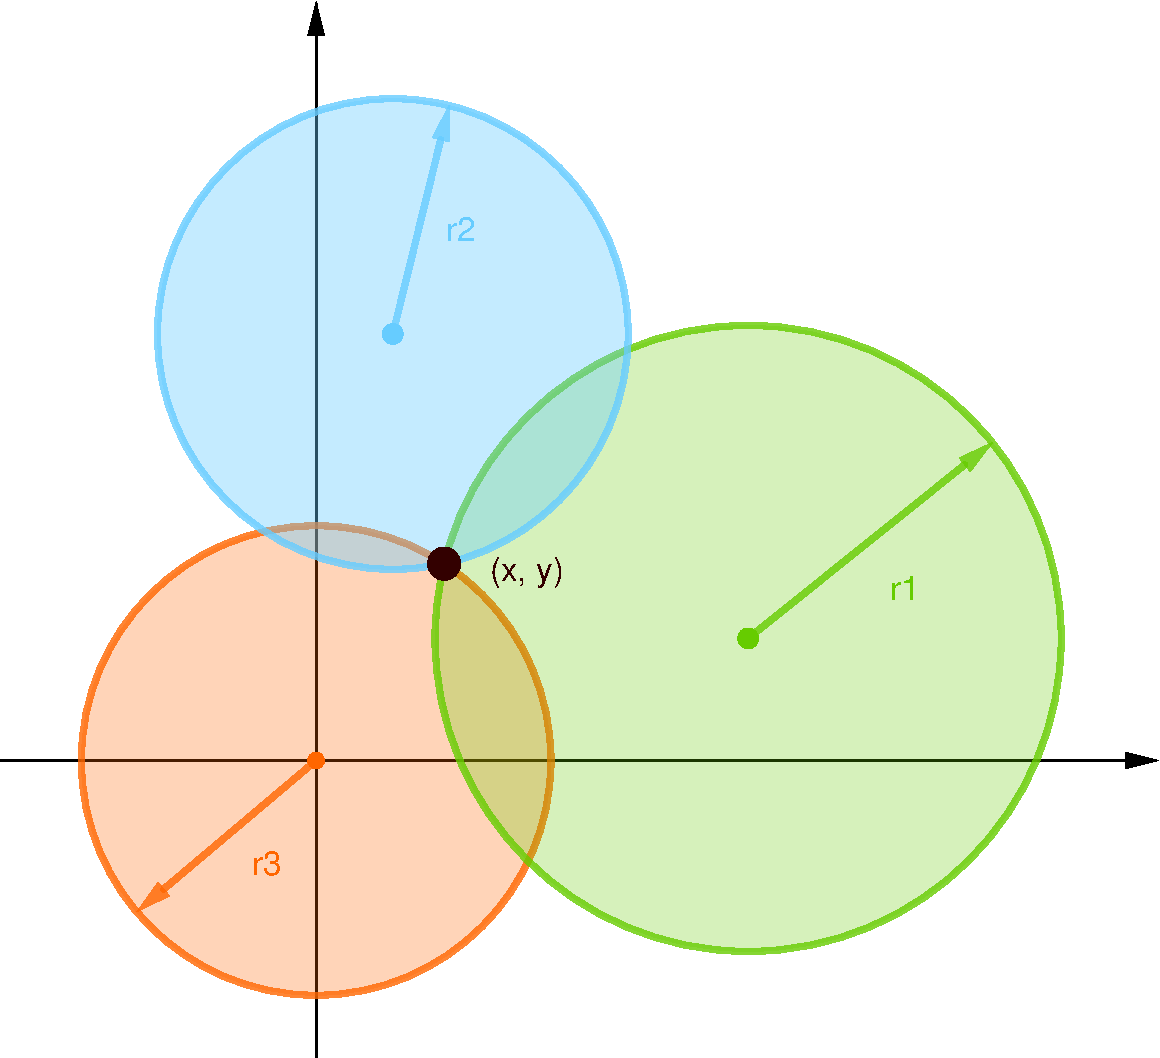
\includegraphics[height=\textheight/3]{trilaterazione-caso-ideale}
	\caption{Le coordinate del nodo target si trovano nel punto di intersezione dei tre cerchi}
	\label{fig:trilaterazione-caso-ideale}
\end{figure}

In pratica, tuttavia, le stime della distanza non sono mai così perfette e non viene quasi mai ottenuto un unico punto come intersezione. È più probabile che il nodo target si trovi all'interno di un’area di intersezione tra i cerchi, o è addirittura possibile che i cerchi non si tocchino. Per ovviare a questi inconvenienti si utilizzano dei piccoli accorgimenti al metodo tradizionale della Trilaterazione. Questo metodo che andremo a descrivere viene realizzato iterativamente per tutti e tre i nodi beacon.
\begin{enumerate}
	
	\item Vengono disegnati due cerchi attorno a due nodi beacon a scelta;
	
	\item Se il punto di intersezione è unico, si salvano le coordinate di questo;
	
	\item Se i due cerchi non si toccano, vengono aumentati i raggi in maniera proporzionale in modo che si tocchino in un unico punto;
	
	\item Se i due cerchi non si toccano in due punti, viene considerato quello che ha distanza dal terzo nodo beacon più vicina alla stima della distanza calcolata per questo nodo;
	
	\item Alla fine di questo procedimento, iterato per tutti e tre i nodi, viene calcolata la media delle coordinate, che corrispondono alla posizione stimata del nodo.
	
\end{enumerate}
Questo algoritmo è leggermente più complesso, almeno in linea di principio, ma offre performance migliori. In figura \ref{fig:trilaterazione-raffinamento-passo-1}, figura \ref{fig:trilaterazione-raffinamento-passo-2} e figura \ref{fig:trilaterazione-raffinamento-passo-3} è mostrato come opera questo adattamento dell’algoritmo di Trilaterazione.

\begin{figure}[htp]
	\centering
	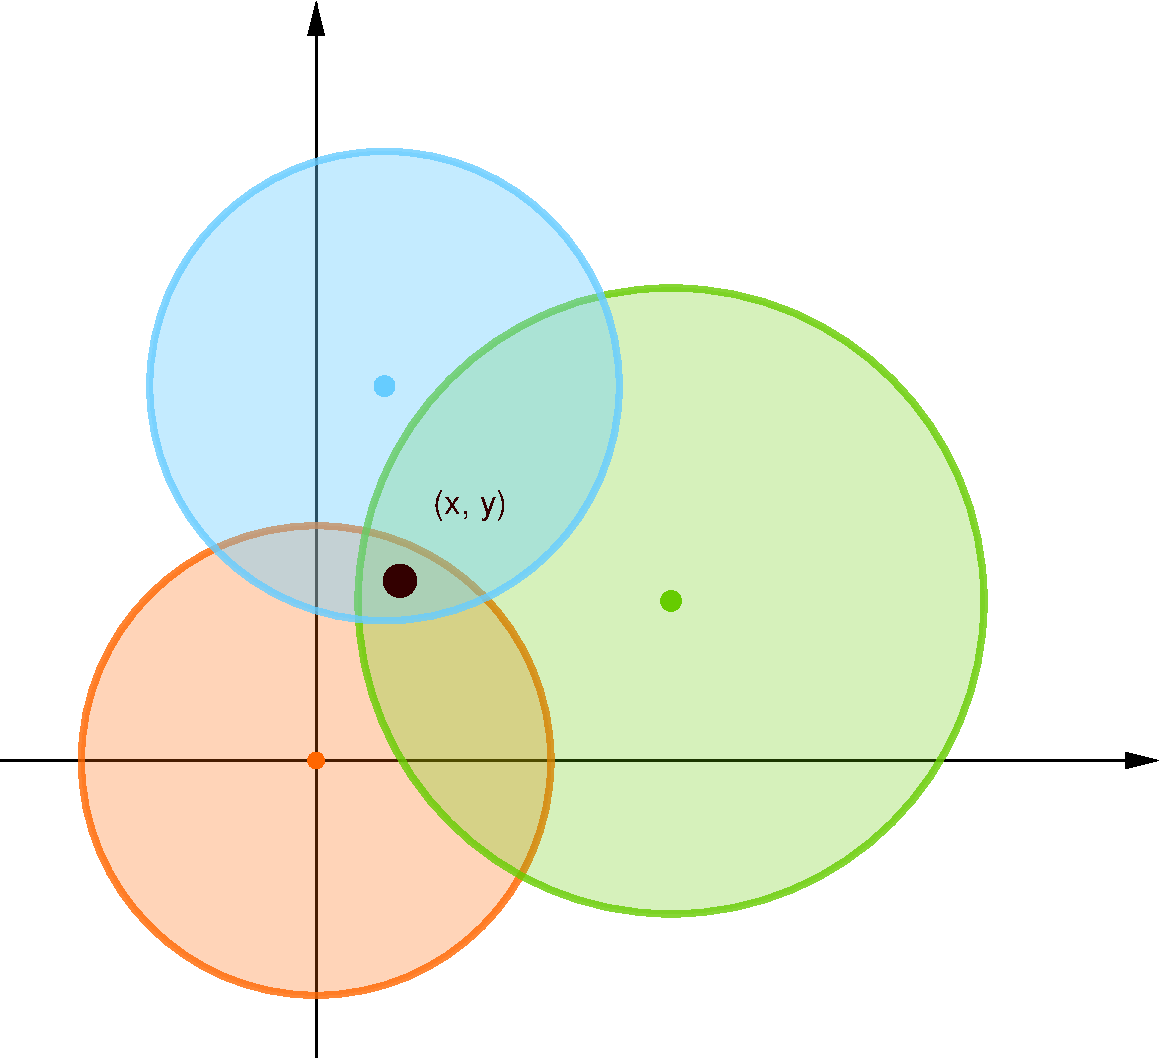
\includegraphics[height=\textheight/3]{trilaterazione-raffinamento-passo-1}
	\caption{Esempio del caso in cui il punto di intersezione non sia unico.}
	\label{fig:trilaterazione-raffinamento-passo-1}
\end{figure}

\begin{figure}[htp]
	\centering
	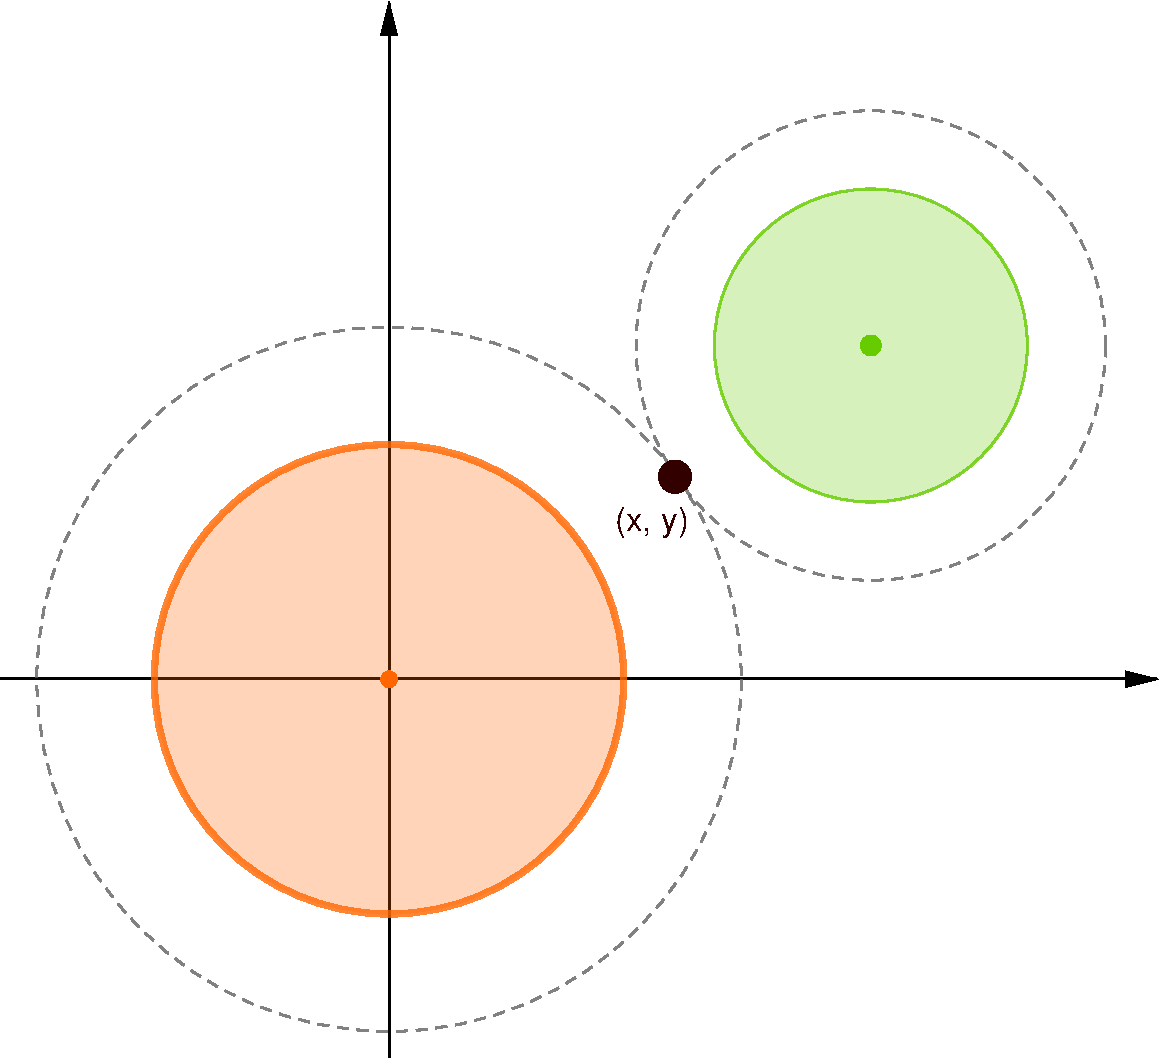
\includegraphics[height=\textheight/3]{trilaterazione-raffinamento-passo-2}
	\caption{Esempio del caso in cui i cerchi non si tocchino. Vengono aumentati i raggi in maniera proporzionale fin quando non si raggiunge il punto di incontro.}
	\label{fig:trilaterazione-raffinamento-passo-2}
\end{figure}

\begin{figure}[htp]
	\centering
	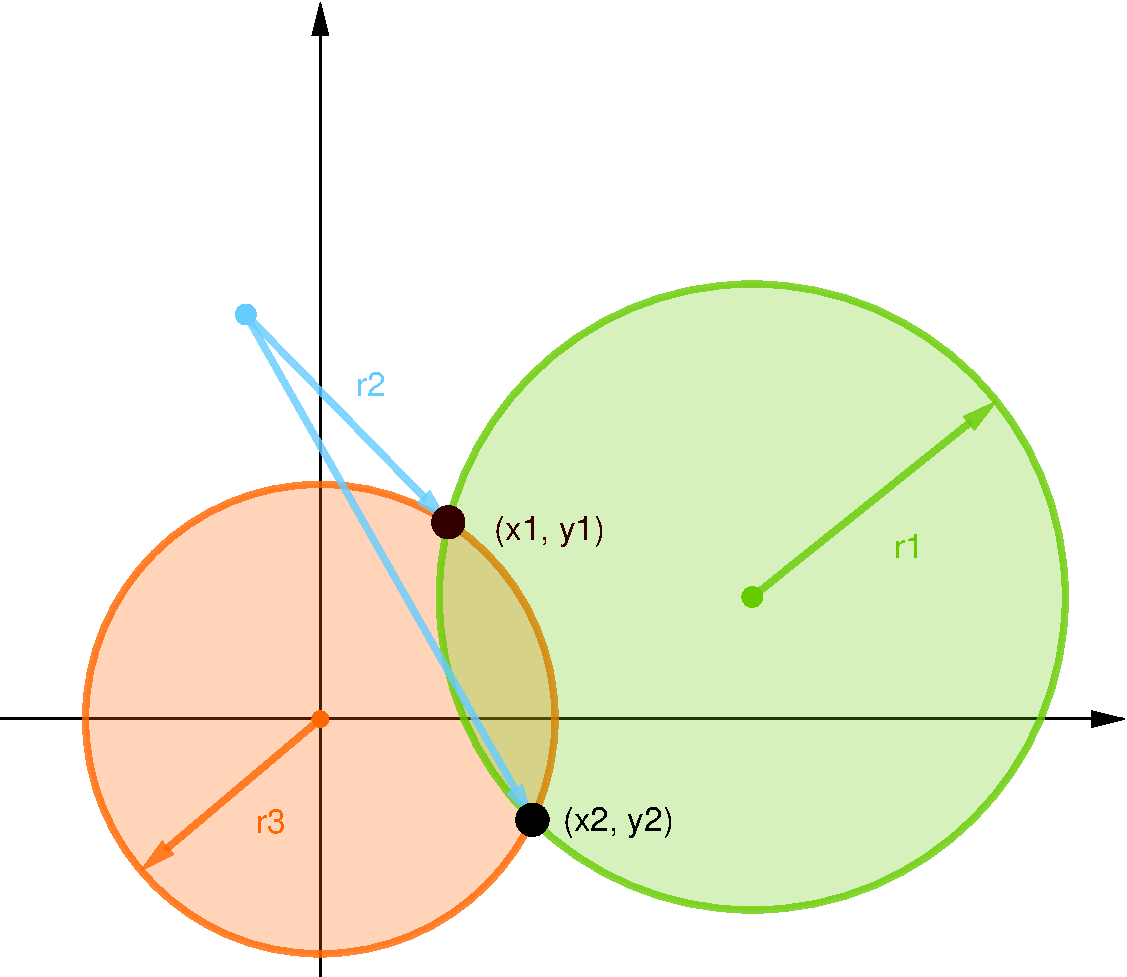
\includegraphics[height=\textheight/3]{trilaterazione-raffinamento-passo-3}
	\caption{Esempio del caso in cui vi siano due punti di intersezione. Il punto tenuto in considerazione è quello con distanza più vicina a quella stimata.}
	\label{fig:trilaterazione-raffinamento-passo-3}
\end{figure}			% progetto
	% !TEX encoding = UTF-8
% !TEX TS-program = pdflatex
% !TEX root = ../tesi.tex
% !TEX spellcheck = it-IT

%*************************************************************
\chapter{Progetto}
\label{cap:progetto}
%*************************************************************

La fase di progettazione del sistema si è svolta partendo dall'analisi dei requisiti del progetto sulla base di tecnologie preesistenti. I vincoli e gli obiettivi del progetto sono stati definiti all’inizio dell’esperienza di tirocinio, svolta all'interno della società Evomatic s.r.l. di Rovigo.

\section{Situazione preesistente}
La società Evomatic s.r.l. è una società che commercializza la propria piattaforma web per la gestione e il tracciamento delle risorse in movimento. La piattaforma utilizza in modo massivo la tecnologia GPS per il tracciamento delle risorse in campo aperto. Il tracciamento delle risorse, sprovviste di tecnologia GPS, può avvenire tramite l'installazione di opportuni moduli GPS oppure si può utilizzare direttamente l'antenna GPS di uno smartphone Android.
L'invio dei dati di posizione delle risorse verso la piattaforma avviene in entrambi i casi sfruttando la connessione internet dello smartphone Android. Oltre alla tracciabilità delle risorse, la piattaforma offre la possibilità di fornire un controllo sui mezzi. Il controllo sui mezzi è possibile tramite l’uso di TAG BLE, che implementano, tramite un'applicazione Android che si interfaccia con la piattaforma, le funzionalità di identificazione dell'utilizzatore della risorsa consentendo, o meno, di usare le funzionalità della risorsa.

\section{Specifiche del progetto}
La piattaforma esistente sfrutta la tecnologia GPS per la tracciabilità delle risorse in campo aperto. La società Evomatic s.r.l. ha espresso l'esigenza di avere la possibilità di estendere le funzionalità della piattaforma anche in ambiente indoor, utilizzando la maggior parte delle tecnologie impiegate per l'uso in campo aperto.
L'obiettivo del progetto è di realizzare un sistema software per il tracciamento indoor delle risorse, con utilizzo della tecnologia BLE (\emph{Bluetooth Low Energy}).

\section{Vincoli del progetto}
I vincoli del sistema sono stati definiti attraverso vari incontri con il responsabile area ricerca e sviluppo e con il tutor aziendale. Al termine di questi incontri sono state stilate le caratteristiche che deve avere il sistema:
\begin{itemize}
	
	\item Il sistema deve avere un'interfaccia web, che consenta la configurazione e la gestione dei TAG BLE, che operano come beacon, in un ambiente indoor;
	
	\item Il sistema, tramite l'interfaccia web, deve dare la possibilità di visualizzare le varie risorse in movimento all'interno dell'ambiente indoor;
	
	\item Il sistema deve implementare un'applicazione su smartphone Android che consenta di identificare la risorsa e di avviarne o meno il tracciamento;
	
	\item L'applicazione Android deve essere ottimizzata per consentire l'utilizzo dell'applicazione in modo che lo smartphone, con batteria iniziale totalmente carica, non esaurisca tutta la carica a disposizione prima di 8 ore di attività continua;
	
	\item L'applicazione Android deve trasmettere in tempo reale la propria posizione sfruttando la connessione internet dello smartphone e se, per qualsiasi motivo, la connessione internet viene a mancare, il dispositivo Android deve poter bufferizzare i dati rilevati per poi inviarli appena possibile;
	
	\item Tutti i dati riguardanti la posizione di ogni risorsa devono essere memorizzati in un database. Il motore di database, per mantenere la compatibilità con il database esistente della piattaforma, dev'essere Microsoft SQL Server.
	
\end{itemize}

\section{Architettura del sistema}
\label{par:architettura-del-sistema}
L'architettura del sistema progettata per la localizzazione indoor utilizzando TAG BLE e smartphone Android è schematizzata in figura \ref{fig:architettura-sistema}. Rispettando i vincoli di progetto, si sono progettati: il database centrale, l’applicazione Android, il broker MQTT, il localizzatore, il web service e la single page application.

\begin{figure}[htp]
	\centering
	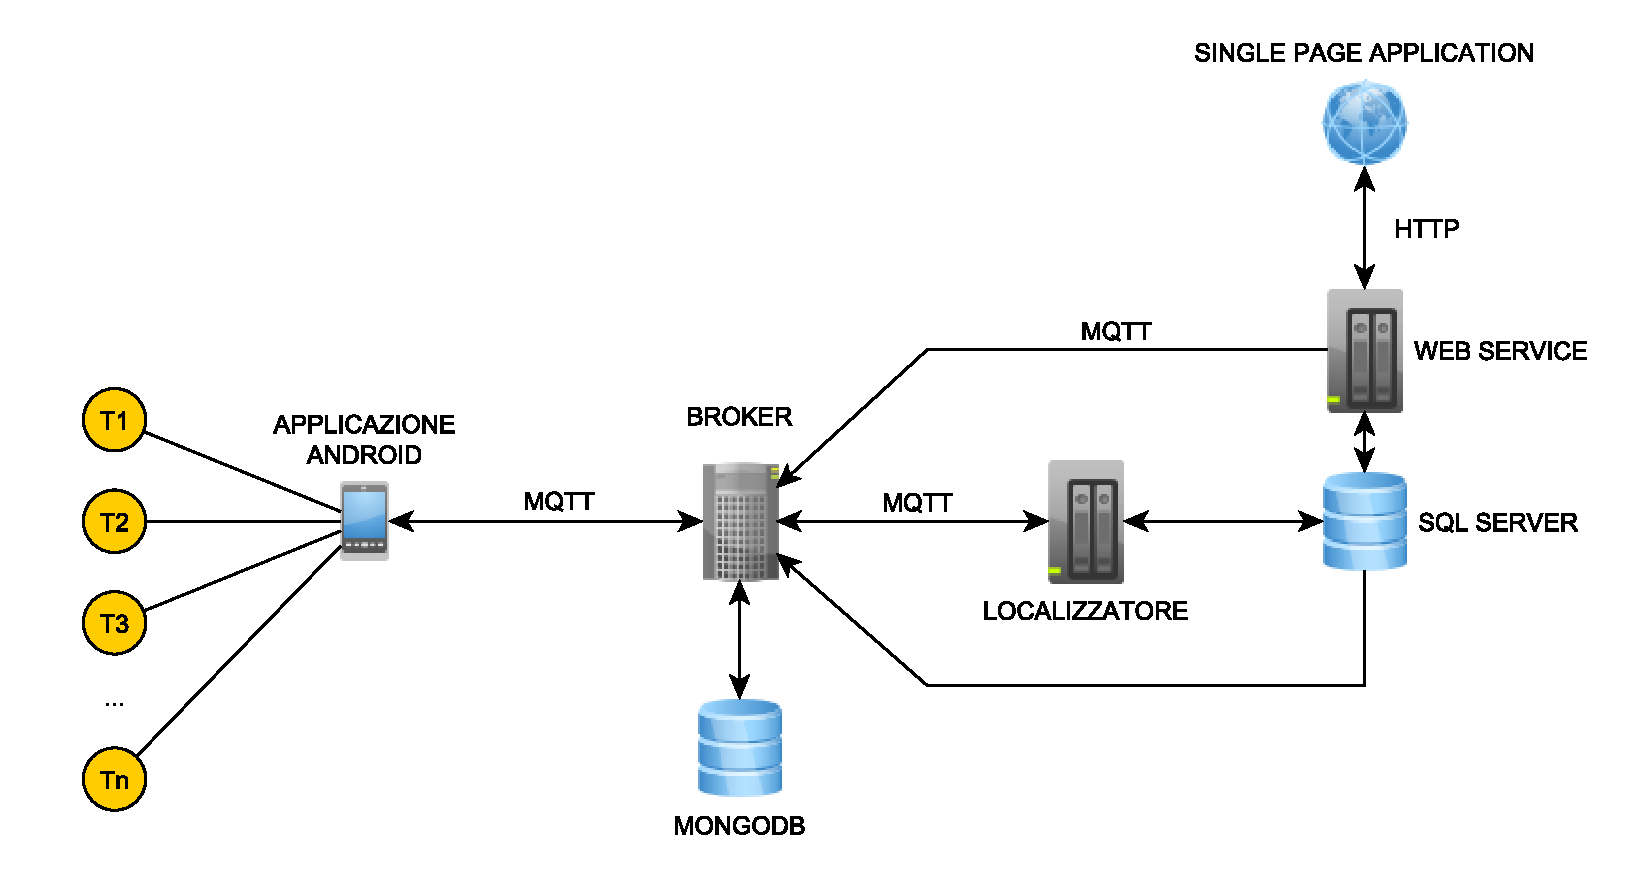
\includegraphics[height=5.4 cm]{architettura-sistema}
	\caption{Architettura del sistema progettato}
	\label{fig:architettura-sistema}
\end{figure}			% RSSI
	% !TEX encoding = UTF-8
% !TEX TS-program = pdflatex
% !TEX root = ../tesi.tex
% !TEX spellcheck = it-IT

%*************************************************************
\chapter{Tecnologie utilizzate}
\label{cap:tecnologie-utilizzate}
%*************************************************************

La tecnologia principale con cui viene effettuata la stima della distanza è la tecnologia BLE. La tecnologia BLE è presente sia sui TAG, dislocati nell'ambiente indoor, sia sullo smartphone, usato per identificare la risorsa in movimento. Per lo sviluppo dell'applicazione sullo smartphone si è analizzata la struttura del sistema Android per poi implementare l'applicazione in linguaggio Java. La scelta dei protocolli da utilizzare a livello applicativo è ricaduta su HTTP, per le comunicazioni effettuate attraverso l'interfaccia web, e MQTT, per le comunicazioni effettuate attraverso lo smartphone Android. I fattori che hanno portato a scegliere MQTT, rispetto ad altri protocolli, sono la leggerezza e l'affidabilità oltre al fatto di essere uno standard definito e aperto.

Per lo sviluppo dei vari componenti si è utilizzato Node.js, runtime Javascript costruito sul motore JavaScript V8 di Google Chrome.

I database utilizzati per la memorizzazione dei dati sono di tipo relazionale e in particolare si è utilizzato SQLite per la memorizzazione dei dati nel sistema Android mentre si è utilizzato Microsoft SQL Server per la memorizzazione delle posizioni di tutte le risorse.

Dato che si sono utilizzati database relazionali, SQLite per Android e Microsoft SQL Server per la gestione della persistenza del sistema, per le interrogazioni si utilizza il linguaggio SQL.

Per l'applicazione web si è scelto l'approccio \emph{Single Page Application} con il fine di favorire l'interattività. Per realizzare l'interfaccia web si sono utilizzate diverse tecnologie, quali: HTML, CSS, AJAX, Canvas.

Il formato comune utilizzato per l'interscambio dei dati tra i vari componenti è il JSON.

Di seguito si descrivono brevemente le varie tecnologie utilizzate.

\section{Bluetooth}
Nelle telecomunicazioni, Bluetooth \cite{wiki:bluetooth} è uno standard tecnico-industriale di trasmissione dati per reti personali senza fili. Fornisce un metodo standard, economico e sicuro per scambiare informazioni tra dispositivi diversi attraverso una frequenza radio sicura a corto raggio.
La specifica Bluetooth è stata sviluppata da Ericsson e in seguito formalizzata dalla Bluetooth Special Interest Group (SIG). Il protocollo Bluetooth opera nel campo di frequenze assegnato intorno ai 2,45 GHz. Per ridurre le interferenze il protocollo divide la banda in 79 canali e provvede a commutare tra i vari canali 1.600 volte al secondo (frequency hopping).

Nel corso degli anni sono state emesse diverse versioni del protocollo ognuna delle quali implementa diverse specifiche. Ogni dispositivo Bluetooth è configurabile per cercare costantemente altri dispositivi e per collegarsi a questi.

\subsection{Bluetooth 4.0 e BLE}
In data 6 luglio 2010 sono diventate definitive le specifiche della versione 4.0.

Rispetto alle versioni precedenti, la versione 4.0 punta alla riduzione dei consumi energetici. L'obiettivo principale di questa funzionalità opzionale, denominato Low Energy (LE), tramite un'ottimizzazione della struttura di trama e l'impiego di dispositivi più efficienti, comporta una riduzione della velocità, che in questa modalità si attesta a 1 Mbps. In termini trasmissivi, sono stati potenziati i meccanismi di rilevazione e correzione di errore e di cifratura del segnale col supporto di AES-128.

\subsection{TAG BLE}
Un TAG BLE \cite{globaltag:tagble} è un beacon BLE che può contenere, inoltre, un accelerometro, un sensore di temperatura e di umidità. In figura \ref{fig:tag-ble} è possibile vedere com'è fatto un TAG BLE commercializzato da Global Tag.

Un TAG BLE dispone di un pulsante ON/OFF che consente di attivare o disattivare il tag, al fine di permettere all’utente di risparmiare la batteria, qualora non abbia la necessità di mantenere il tag acceso. La distanza di lettura arriva fino a 90 metri. I diversi parametri del beacon BLE, come l’intervallo di emissione, la potenza del segnale, il ``friendly name'' si possono configurare tramite software.

\begin{figure}[htp]
	\centering
	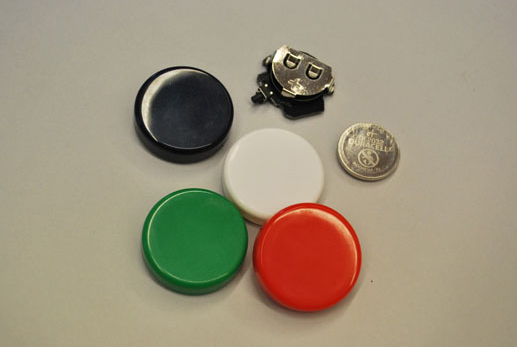
\includegraphics[height=\textheight/3]{tag-ble}
	\caption{TAG BLE}
	\label{fig:tag-ble}
\end{figure}

\section{Il sistema Android}
Android \cite{android:site} è un sistema operativo per dispositivi mobili sviluppato da Google Inc. basato sul kernel Linux. È un sistema embedded progettato principalmente per smartphone e tablet.

Lo sviluppo di Android prosegue attraverso l'Android Open Source Project il quale è software libero ad esclusione di diversi firmware non-liberi inclusi per i produttori di dispositivi e delle cosiddette ``Google Apps'' come ad esempio Google Play. È distribuito sotto i termini della licenza libera Apache 2.0 riservandosi di non-includere software coperto da licenze copyleft.

Android è costituito da un kernel Linux 2.6 e 3.x (da Android 4.0 in poi), con middleware, Librerie e API scritte in C (o C++) e software in esecuzione su un framework di applicazioni che include librerie Java compatibili con librerie basate su Apache Harmony.

La piattaforma hardware principale di Android è l'architettura ARM mentre le applicazioni Android sono Java-based. L'architettura software del sistema Android è schematizzata in figura \ref{fig:architettura-android}.

\begin{figure}[htp]
	\centering
	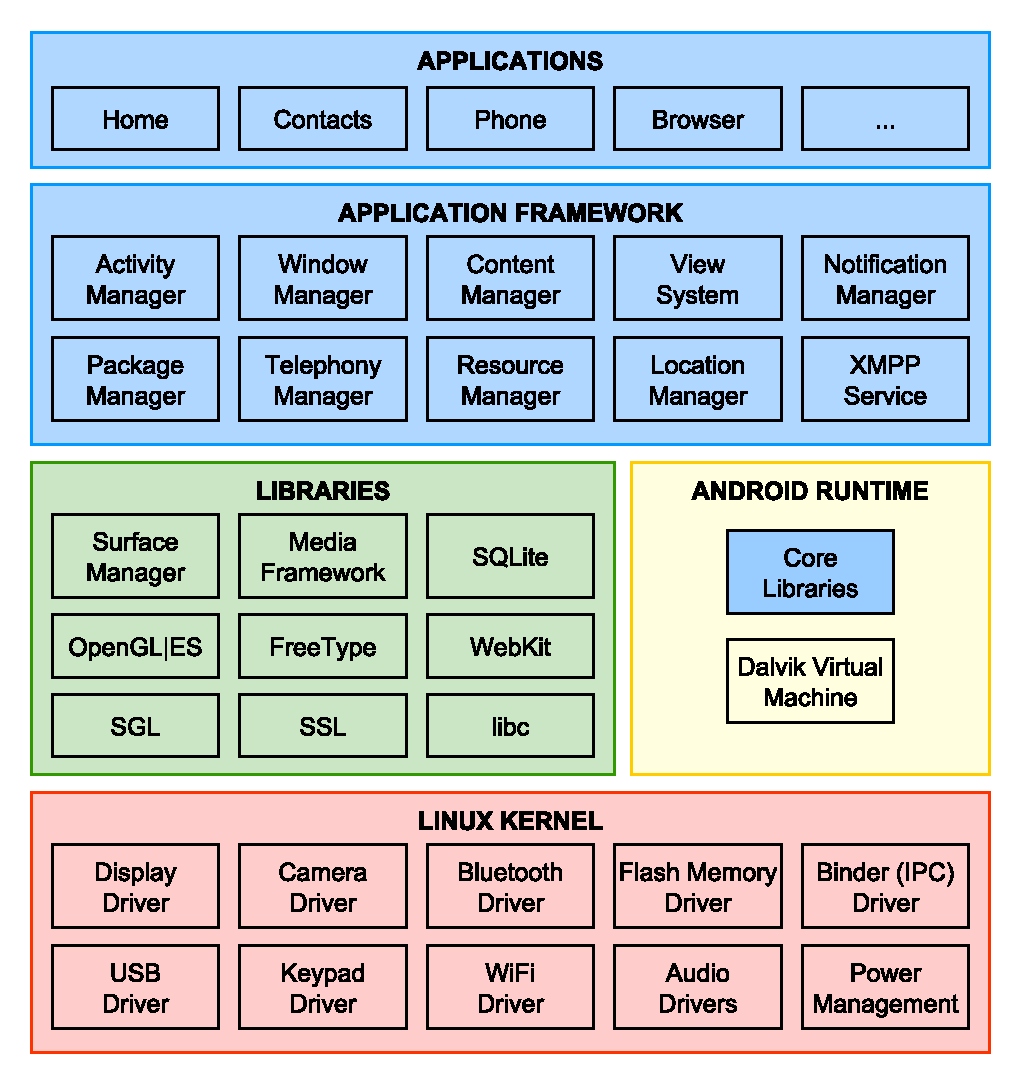
\includegraphics[height=\textheight/3]{architettura-android}
	\caption{Architettura del sistema Android}
	\label{fig:architettura-android}
\end{figure}

\section{Protocolli}

\subsection{MQTT}
MQ Telemetry Transport (MQTT) \cite{mqtt:site} è un protocollo ISO standard di messaggistica leggero di tipo publish-subscribe posizionato in cima a TCP/IP. Il protocollo è stato inventato da Andy Stanford-Clark di IBM, e Arlen Nipper di Cirrus Link Solutions nel 1999.

MQTT è stato progettato per avere bassa latenza, messaggistica sicura su reti fragili e una  distribuzione efficiente a uno o più ricevitori. Il protocollo si concentra sulla riduzione al minimo della quantità di byte necessari per l’invio del messaggio e sul basso consumo energetico. La dimensione massima dei messaggi di 256 mb, quindi non è possibile inviare per ogni messaggio grandi quantità di dati ma è possibile inviare un numero elevato di messaggi di dimensioni ridotte. MQTT fornisce, inoltre, un canale di comunicazione bidirezionale. Questo protocollo viene utilizzato in situazioni in cui è richiesto un basso impatto e dove la banda è limitata. Per poter essere utilizzato il pattern publish-subscribe richiede un \emph{message broker} il quale è responsabile della distribuzione dei messaggi ai client destinatari.

\subsection{HTTP}
L'HyperText Transfer Protocol (HTTP) \cite{HTTP:site} è un protocollo a livello applicativo usato come principale sistema per la trasmissione d'informazioni sul web ovvero in un'architettura tipica client-server. Le specifiche del protocollo sono gestite dal World Wide Web Consortium (W3C). Un server HTTP generalmente resta in ascolto delle richieste dei client sulla porta 80 usando il protocollo TCP a livello di trasporto.
Nell'HTTP le connessioni vengono generalmente chiuse una volta che una particolare richiesta, o una serie di richieste correlate, è stata soddisfatta.

\subsection{MQTT vs HTTP}
Uno dei fattori per cui si è scelto MQTT nell’applicazione Android è dato dal minor consumo di batteria e alla maggiore leggerezza ed affidabilità nella connessione. In tabella \ref{tab:https-vs-mqtt} vengono riportati i risultati di un test \cite{nicholas:https-vs-mqtt} di spedizione di 1024 messaggi con payload di 1 byte. Come si può notare dai dati in tabella utilizzando MQTT si ha una totale consegna dei messaggi inviati oltre avere un consumo di batteria inferiore per ogni messaggio inviato rispetto ad HTTPS.

\begin{table}
	\caption{Test di spedizione di 1024 messaggi con payload da 1 byte con HTTPS e MQTT}
	\label{tab:https-vs-mqtt}
	\begin{center}
		\begin{tabular}{lcccc}
			\toprule
			\textbf{Connessione} 				& \multicolumn{2}{c}{3G} & \multicolumn{2}{c}{Wifi} \\
			\midrule
			\textbf{Protocollo} 				& HTTPS 		& MQTT 			& HTTPS 		& MQTT \\
			\midrule
			\textbf{\% Batteria / Ora} 			& 18.43\% 		& 16.13\% 		& 3.45\% 		& 4.23\% \\
			\textbf{Messaggi / Ora} 			& 1708 			& 160278 		& 3628 			& 263314 \\
			\textbf{\% Batteria / Messaggio} 	& 0.01709 		& 0.00010 		& 0.00095		& 0.00002 \\
			\textbf{Messaggi Ricevuti} 			& 240/1024 		& 1024/1024 	& 524/1024 		& 1024/1024 \\
			\bottomrule
		\end{tabular}
	\end{center}
\end{table}


\section{NodeJS}
Node.js \cite{node:site} è un runtime Javascript costruito sul motore JavaScript V8 di Google Chrome. Il modello utilizzato da Node.js è il modello I/O non bloccante ad eventi, che lo rende un framework leggero ed efficiente. Il modello I/O non bloccante richiede al sistema operativo di ricevere notifiche al verificarsi di determinati eventi, rimanendo quindi in sleep fino alla notifica stessa. Quando la notifica avviene, allora il sistema operativo torna attivo per eseguire le istruzioni previste nella funzione di callback, funzione che viene eseguita una volta che il risultato dell'elaborazione da parte del sistema operativo è disponibile.

Node.js è organizzato in moduli i quali sono scritti in JavaScript. Ogni sviluppatore può scrivere nuovi moduli in JavaScript oppure può includere dei moduli già scritti prelevandoli da npm, gestore dei pacchetti predefinito di Node.js.

\section{JavaScript}
JavaScript \cite{javascript:site} è un linguaggio di scripting orientato agli oggetti e agli eventi, comunemente utilizzato nella programmazione Web lato client per la creazione, in siti web e applicazioni web, di effetti dinamici interattivi tramite funzioni di script invocate da eventi innescati a loro volta in vari modi dall'utente sulla pagina web in uso. Tali funzioni di script, utilizzati dunque nella logica di presentazione, possono essere opportunamente inserite in file HTML. JavaScript è stato standardizzato per la prima volta il 1997 dalla ECMA con il nome ECMAScript ed è, inoltre, uno standard ISO.

\section{SQL}
SQL (Structured Query Language) \cite{wiki:sql} è un linguaggio standardizzato per database basati sul modello relazionale (RDBMS) progettato per:
\begin{itemize}
	
	\item Creare e modificare schemi di database (Data Definition Language);
	
	\item Inserire, modificare e gestire dati memorizzati (Data Manipulation Language);
	
	\item Interrogare i dati memorizzati (Data Query Language);
	
	\item Creare e gestire strumenti di controllo ed accesso ai dati (Data Control Language).
	
\end{itemize}
SQL non è solo di un semplice linguaggio di interrogazione, ma alcuni suoi sottoinsiemi si occupano della creazione, della gestione e dell'amministrazione del database.

\section{Single Page Application}
Con Single Page Application \cite{wiki:single-page-application} si intende un'applicazione web che può essere usata o consultata su una singola pagina web con l'obiettivo di fornire un'esperienza utente più fluida, simile alle applicazioni desktop dei sistemi operativi tradizionali. In un'applicazione su singola pagina tutto il codice necessario è recuperato in un singolo caricamento della pagina mentre le risorse appropriate sono caricate dinamicamente e aggiunte alla pagina quando necessario, di solito in risposta ad azioni dell'utente. In particolare, la pagina non si ricarica in nessun punto del processo, né lascia il controllo a un'altra pagina. Di seguito si presentano brevemente le tecnologie con cui si sviluppa un'applicazione web di questo tipo.

\subsection{HTML}
L'HTML (HyperText Markup Language) \cite{HTML:site} è un linguaggio di markup. Nato per la formattazione e impaginazione di documenti ipertestuali disponibili nel web 1.0, oggi è utilizzato principalmente per il disaccoppiamento della struttura logica di una pagina web. L'HTML è un linguaggio di pubblico dominio, la cui sintassi è stabilita dal World Wide Web Consortium (W3C). È derivato da SGML, un metalinguaggio finalizzato alla definizione di linguaggi utilizzabili per la stesura di documenti destinati alla trasmissione in formato elettronico.

\subsection{CSS}
Il CSS (Cascading Style Sheets) \cite{CSS:site} è un linguaggio usato per definire la formattazione di documenti HTML, XHTML e XML. L'introduzione del CSS si è resa necessaria per separare i contenuti delle pagine HTML dalla loro formattazione e permettere una programmazione più chiara e facile da utilizzare, sia per gli autori delle pagine stesse sia per gli utenti, garantendo contemporaneamente anche il riutilizzo di codice e una sua più facile manutenzione.

\subsection{AJAX}
AJAX (Asynchronous JavaScript and XML) \cite{AJAX:site} è una tecnica di sviluppo software per la realizzazione di applicazioni web interattive. Lo sviluppo di applicazioni HTML con AJAX si basa su uno scambio di dati in background fra web browser e server, che consente l'aggiornamento dinamico di una pagina web senza esplicito ricaricamento da parte dell'utente. AJAX è asincrono nel senso che i dati extra sono richiesti al server e caricati in background senza interferire con il comportamento della pagina esistente. Normalmente le funzioni richiamate sono scritte con il linguaggio JavaScript. Tuttavia, l'uso di JavaScript e di XML non è obbligatorio, come non è detto che le richieste di caricamento debbano essere necessariamente asincrone.

\section{JSON}
JSON (JavaScript Object Notation) \cite{json:site} è un formato adatto all'interscambio di dati fra applicazioni client-server. È basato sul linguaggio JavaScript Standard ECMA-262 3\ap{a} edizione dicembre 1999, ma ne è indipendente. Viene usato in AJAX come alternativa a XML/XSLT.			% scelta tecnologie
	% !TEX encoding = UTF-8
% !TEX TS-program = pdflatex
% !TEX root = ../tesi.tex
% !TEX spellcheck = it-IT

%*************************************************************
\chapter{Implementazione del sistema}
\label{cap:implementazione}
%*************************************************************

Questo capitolo descrive la fase dello sviluppo del sistema, partendo dall'architettura presentata nel paragrafo \ref{par:architettura-del-sistema}, per poi scendere nel dettaglio dei vari componenti.

\section{Sviluppo componenti del sistema}
Coerentemente con l'architettura illustrata in figura \ref{fig:architettura-sistema} si è implementato ogni componente del sistema. Per lo sviluppo dei vari componenti si sono utilizzati dei framework. In figura \ref{fig:color-coded} si riporta il grafico color coded dei vari componenti del sistema dove in azzurro sono evidenziate le parti sviluppate mentre in verde sono indicati i framework e i moduli utilizzati. Di seguito si descrive, in ordine di sviluppo, l’implementazione di ogni componente del sistema.

\begin{figure}[htp]
	\centering
	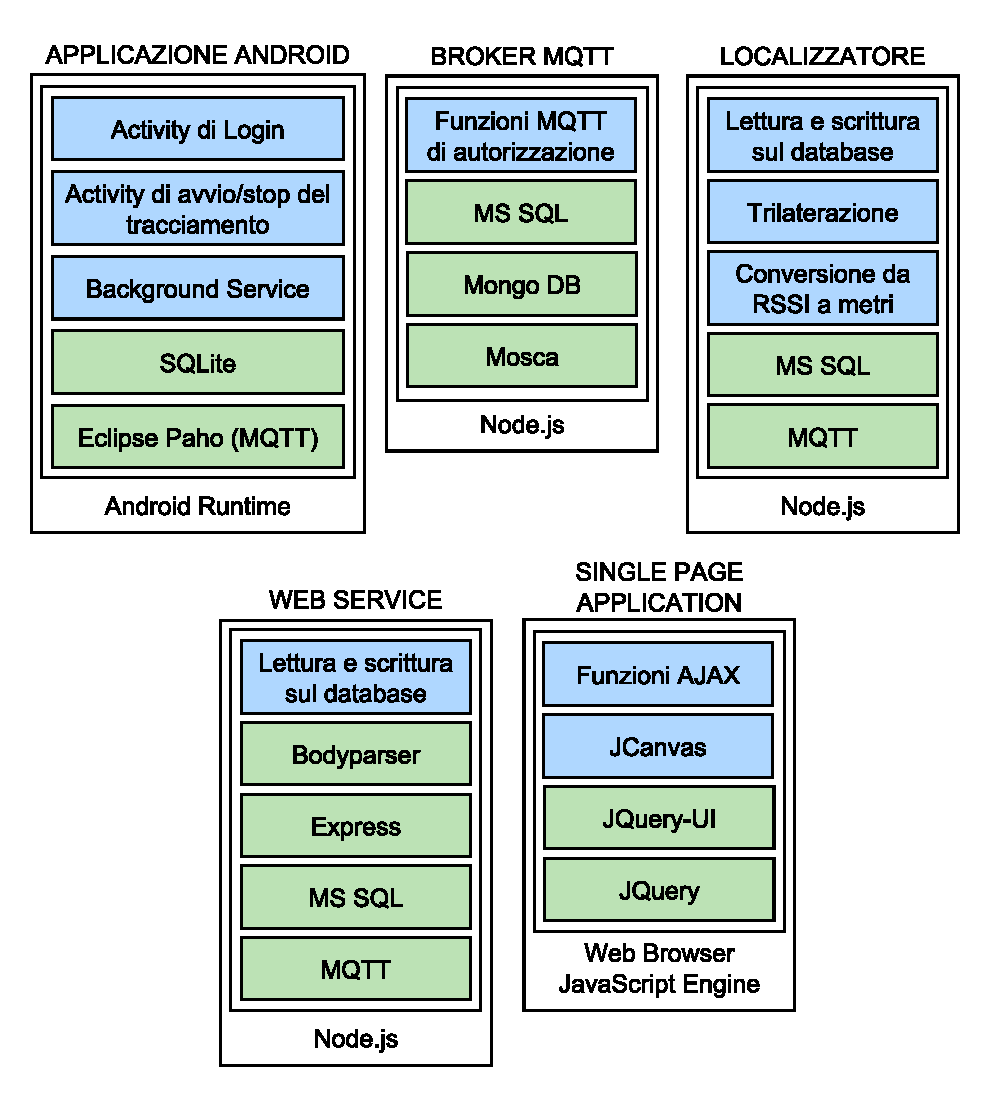
\includegraphics[height=10 cm]{color-coded}
	\caption{Grafico color coded dei componenti sviluppati}
	\label{fig:color-coded}
\end{figure}

\section{Database}
Il motore del database centrale è Microsoft SQL Server, coerentemente con quanto imposto nei vincoli di progetto. Per l’immagazzinamento dei dati si è realizzato il modello entità-relazione rappresentato in figura \ref{fig:modello-er-db-centrale}. Il database contiene quattro entità in relazione tra loro. Le entità sono:
\begin{description}
	
	\item[UTENTE] si occupa di memorizzare i dati relativi ad un utente che può accedere al sistema;
	
	\item[TRACCIA] si occupa di memorizzare le tracce dei vari utenti;
	
	\item[POSIZIONE] contiene per ogni traccia le coordinate dell'ambiente indoor;
	
	\item[TAG BLE] contiente le informazioni riguardanti la posizione di ogni TAG BLE.
	
\end{description}
Le relazioni che intercorrono tra le entità sono:
\begin{description}
	
	\item[Registra] per ogni utente possono essere presenti una o più tracce con datetime diverso per ogni traccia.
	
	\item[Corrisponde] ad ogni traccia applicando l'algoritmo di trilaterazione corrsiponde una sola posizione e viceversa;
	
	\item[Contiene] ogni traccia contiene 3 TAG BLE i quali possono avere valori di RSSI diversi ed ogni TAG BLE può essere presente in più tracce;
	
\end{description}
Utilizzando il modello ER appena presentato si è costruito il modello relazionale e, infine, si è applicata la procedura di normalizzazione per minimizzare la ridondanza dei dati.

\begin{figure}[htp]
	\centering
	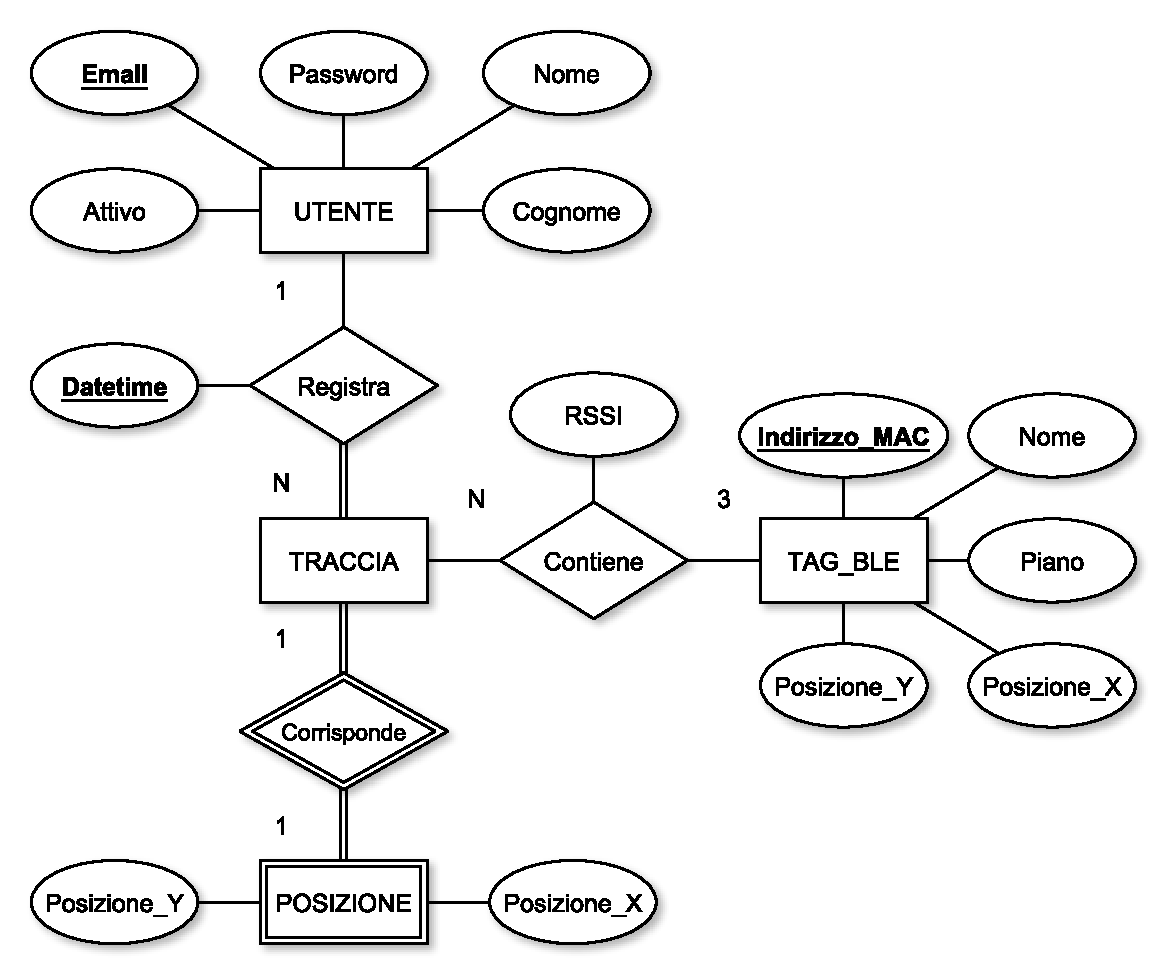
\includegraphics[height=\textheight/3]{modello-er-db-centrale}
	\caption{Modello E-R del database centrale}
	\label{fig:modello-er-db-centrale}
\end{figure}

\section{Broker MQTT}
Per lo sviluppo del broker MQTT si è scelto di utilizzare il broker Mosca. Mosca \cite{mosca:site} è un broker MQTT che può essere integrato in applicazioni Node.js. Il broker implementa diverse caratteristiche, tra cui: MQTT 3.1 e 3.1.1, QoS 0 e QoS 1, varie opzioni di archiviazione per i pacchetti offline QoS 1 e le sottoscrizioni. Per avere la garanzia nella comunicazione, si deve utilizzare un database. Mosca offre la compatibilità con diversi database non relazionali. Si è scelto di utilizzare il database MongoDB che si occuperà di rendere disponibili le funzioni di:
\begin{description}
	
	\item[Keep-Alive message] il broker riesce a identificare una disconnessione non esplicita del client;
	
	\item[Will message] viene impostato nel messaggio di CONNECT con topic, QoS e retain. In caso di disconnessione inaspettata il messaggio ``Will'' viene mandato ai subscribers registrati;
	
	\item[Retain message] un messaggio pubblicato su un topic viene mantenuto sul broker. Un successivo subscriber che si connette sullo stesso topic riceve il messaggio (last known good message).
	
	\item[Persistent Session] dopo la disconnessione del client, tutte le sottoscrizioni vengono mantenute nel broker e recuperate alla connessione successiva.
	
\end{description}
Dopo aver integrato il broker seguendo le linee guida della documentazione, si sono riscritte le funzioni che permettono di verificare se un utente può utilizzare o meno il sistema. La funzione di autenticazione, visibile nel listato \ref{cod:auth-broker}, utilizza la libreria Mssql per interfacciarsi con Microsoft SQL Server.
\begin{lstlisting}[language=JavaScript, label=cod:auth-broker, caption=Funzione di autenticazione del broker MQTT]
// Autenticazione
authenticate = function(client, email, password, callback) {
var autorizzato = false;
return mssql.connect(sqlConfig).then(function() {
var request = new mssql.Request(mssql);
// conta gli utenti che hanno la stessa email e password
var stringRq = "SELECT COUNT(*) AS presente FROM utente WHERE Email = '" + email + "' AND Password = '" + password + "';";
// autorizzo se presente altrimenti rifiuto la connessione
return request.query(stringRq).then(function(result) {
autorizzato = result[0].presente == 1;
if (!autorizzato) { // email non autorizzata
	return callback(null, autorizzato); }
else { // email autorizzata
	client.user = email;
	return callback(null, autorizzato); }
mssql.close(); })
.catch(function (err) {
console.log(err);
mssql.close(); });
}).catch(function (err) {
console.log(err); });
}
\end{lstlisting}

\section{Localizzatore}
Il localizzatore è un componente che si occupa di interfacciarsi con il database utilizzando il protocollo MQTT. Si è utilizzata la libreria MQTT.js che implementa le funzioni del protocollo MQTT per Node.js. Il localizzatore, al suo avvio, deve pubblicare la lista di tutti i TAG BLE presenti nel database centrale con il flag retain.
Quando il broker riceve da un utente un messaggio contenente un insieme di tracce, il broker lo inoltra al localizzatore. Il localizzatore a questo punto, memorizza le tracce ricevute nel database e successivamente effettua prima la conversione da RSSI a metri, poi ottenendo la posizione relativa dei TAG BLE interessati effettua il calcolo della posizione eseguendo l'algoritmo di Trilaterazione.

\subsection{Conversione da RSSI a metri}
La conversione da RSSI a metri si è implementata nel localizzatore con il codice visibile nel listato \ref{cod:rssi-to-meter}, coerentemente con quanto spiegato nel paragrafo \ref{par:ranging}. 

\begin{lstlisting}[language=JavaScript, label=cod:rssi-to-meter, caption=Conversione da RSSI a Metri]
// Conversione da RSSI a Metri
calcoloRssiMetri = function(rssi) {
	var A = -40 // potenza del segnale ricevuto in campo aperto
	var n = 2 // costante di propagazione in campo aperto
	
	var esponente = (A - rssi) / (10 * n);
	return Math.pow(10,esponente);
}
\end{lstlisting}

\subsection{Algoritmo di Trilaterazione}
L'algoritmo di Trilaterazione si è implementato seguendo quanto indicato nel paragrafo \ref{par:trilaterazione}. In primo luogo si implementa una funzione che permetta di calcolare il punto medio di un array di punti. La firma della funzione è visibile nel listato \ref{cod:media-punti}.

\begin{lstlisting}[language=JavaScript, label=cod:media-punti, caption=Calcolo del punto medio]
getMediaPunti = function(punti) { /* ... */ }
\end{lstlisting}

Successivamente si definisce una funzione che ritorna il punto medio della Trilaterazione iterata per tutti e tre i nodi beacon, visibile nel listato \ref{cod:esegui-trilaterazione}.

\begin{lstlisting}[language=JavaScript, label=cod:esegui-trilaterazione, caption=Calcolo del punto medio della Trilaterazione iterata per i tre nodi beacon]
trilaterazione = function(x1, y1, d1, x2, y2, d2, x3, y3, d3) {
	return getMediaPunti(new Array(
	getTrilaterazione(x1, y1, d1, x2, y2, d2, x3, y3, d3),
	getTrilaterazione(x3, y3, d3, x1, y1, d1, x2, y2, d2),
	getTrilaterazione(x2, y2, d2, x3, y3, d3, x1, y1, d1)))
}
\end{lstlisting}


Infine si scrive l'algoritmo di Trilaterazione, visibile nel listato \ref{cod:trilaterazione}, risolvendo il sistema di equazioni \ref{eq:sistema-trilaterazione}.


\begin{lstlisting}[language=JavaScript, label=cod:trilaterazione, caption=Algoritmo di trilaterazione]
getTrilaterazione = function(x1, y1, d1, x2, y2, d2, x3, y3, d3) {
var r = new Object(); // è l'oggetto da ritornare
// verifico se i due cerchi si incrociano
if (Math.sqrt(Math.pow(x1-x2,2) + Math.pow(y1-y2,2)) <= (d1+d2)) {
var a1=-2*x1; var b1=-2*y1; var a2=-2*x2; var b2=-2*y2;
var c1=Math.pow(x1,2)+Math.pow(y1,2)-Math.pow(d1,2);
var c2=Math.pow(x2,2)+Math.pow(y2,2)-Math.pow(d2,2);
if(a1 != a2) { // ricavo le coordinate del polinomio
var a=1+Math.pow(b2-b1,2)/Math.pow(a1-a2,2);
var b=2*(b2-b1)*(c2-c1)/Math.pow(a1-a2,2)+(a1*(b2-b1))/(a1-a2)+b1;
var c=Math.trunc(c1+a1*(c2-c1)/(a1-a2)+Math.pow(c2-c1,2)/Math.pow(a1-a2,2));
// risolvo l'eq. di secondo grado a*x^2 + b*x + c
var delta = Math.sqrt(Math.pow(b,2) - 4*a*c);
var ys1=(-b+delta)/(2*a); var ys2=(-b-delta)/(2*a);
// ricavo i due valori di x risolvendo l'eq.
var xs1=(c2-c1)/(a1-a2)+((b2-b1)*ys1)/(a1-a2);
var xs2=(c2-c1)/(a1-a2)+((b2-b1)*ys2)/(a1-a2);
// se le due soluzioni sono uguali ho il punto di intersezione
if(xs1==xs2 && ys1==ys2) { r.x=xs1; r.y=ys1; return r; }
else { // altrimenti la distanza del nodo stimato dal terzo anchor
d1=Math.sqrt(Math.pow(xs1-x3,2)+Math.pow(ys1-y3,2));
d2=Math.sqrt(Math.pow(xs2-x3,2)+Math.pow(ys2-y3,2));
if ((d1-d3)<(d2-d3)) { r.x=xs1; r.y=ys1; return r; }
else { r.x=xs2; r.y=ys2; return r;}
}}
else { // ricavo le coordinate del polinomio
var a=1+Math.pow(a2-a1,2)/Math.pow(b1-b2,2);
var b=2*(a2-a1)*(c2-c1)/Math.pow(b1-b2,2)+(b1*(a2-a1))/(b1-b2)+a1;
var c=Math.trunc(c1+b1*(c2-c1)/(b1-b2)+Math.pow(c2-c1,2)/Math.pow(b1-b2,2));
// risolvo l'eq. di secondo grado a*x^2 + b*x + c
var delta=Math.sqrt(Math.pow(b,2)-4*a*c);
var xs1=(-b+delta)/(2*a); var xs2=(-b-delta)/(2*a);
// ricavo i due valori di y risolvendo l'eq.
var ys1=(c2-c1)/(b1-b2)+((a2-a1)*xs1)/(b1-b2);
var ys2=(c2-c1)/(b1-b2)+((a2-a1)*xs2)/(b1-b2);
// se le due soluzioni sono uguali ho il punto di intersezione
if(xs1==xs2 && ys1==ys2) { r.x=xs1; r.y= ys1; return r; }
else { // altrimenti la distanza del nodo stimato dal terzo anchor
d1=Math.sqrt(Math.pow(xs1-x3,2)+Math.pow(ys1-y3,2));
d2=Math.sqrt(Math.pow(xs2-x3,2)+Math.pow(ys2-y3,2));
if ((d1-d3)<(d2-d3)) { r.x=xs1;	r.y=ys1; return r; }
else { r.x = xs2; r.y = ys2; return r;}
}}}
else { // altrimenti se i due cerchi non si incrociano
var dr=(Math.sqrt(Math.pow(x1-x2,2)+Math.pow(y1-y2,2))-(d1+d2))/2;
// nuovi raggi
d1 += dr;	d2 += dr;
return getTrilaterazione(x1, y1, d1, x2, y2, d2, x3, y3, d3);
}}
\end{lstlisting}

\section{Web Service}
Il web service si occupa di rendere disponibili le varie funzioni per la Single Page Application. Per lo sviluppo si sono utilizzate le seguenti librerie:
\begin{description}
	
	\item[MQTT.js] per pubblicare al broker MQTT la lista dei TAG BLE, se questi vengono modificati dalla SIngle Page Application, con il flag retain;
	
	\item[Express] per realizzare le varie funzioni REST del webservice;
	
	\item[Body-parser] per effettuare il parsing middleware del corpo del messaggio ricevuto dalla Single Page Application;
	
	\item[Mssql] per interfacciarsi con Microsoft SQL Server.
	
\end{description}
Si sono sviluppate le varie API del web service utilizzando prevalentemente le librerie Express e Mssql, effettuando delle interrogazioni SQL specifiche per poi inviare alla Single Page Application i dati richiesti.


\section{Single Page Application}
La Single Page Application offre all'utente la possibilità di configurare i TAG BLE e di vedere le risorse all'interno dell'ambiente indoor desiderato.
I casi d'uso implementati sono visibili in figura \ref{fig:ucs-spa}.
Per lo sviluppo dell'applicazione si sono utilizzati i seguenti framework:
\begin{description}
	
	\item[JQuery] utilizzato per le chiamate AJAX e per il supporto multibrowser;
	
	\item[JQuery-UI] utilizzato per creare le varie maschere di inserimento e modifica dei dati riguardanti alla configurazione dei TAG BLE;
	
	\item[JCanvas] utilizzato per disegnare sulla mappa dell’ambiente indoor e per animare i movimenti real time delle varie risorse monitorate.
	
\end{description}
Si è utilizzato, inoltre, a corredo dei framework JavaScript sopra citati anche il linguaggio HTML e CSS per definire la struttura e l’aspetto grafico dell'applicazione.

\begin{figure}[htp]
	\centering
	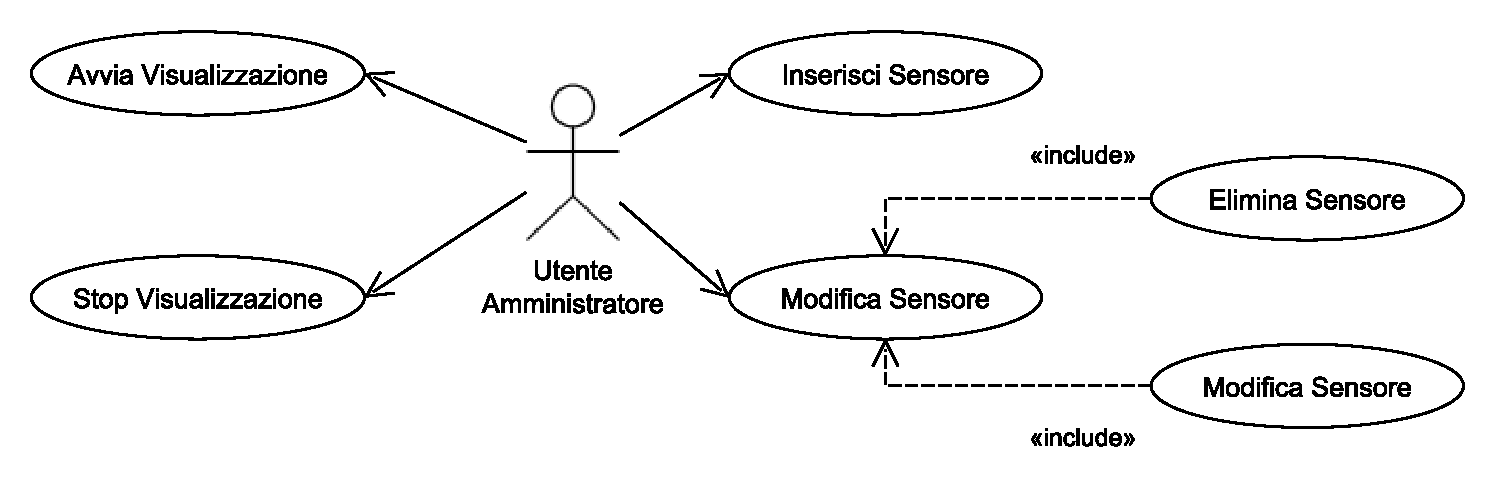
\includegraphics[width=\textwidth]{ucs-spa}
	\caption{Casi d'uso Single Page Application}
	\label{fig:ucs-spa}
\end{figure}

\section{Applicazione Android}
L'applicazione Android contiene due activity: l'activity di login e l'activity per avviare o fermare la rilevazione della risorsa. L’activity di login si interfaccia con l’utente chiedendo di inserire email e password per verificare la possibilità di accedere al sistema. L'activity di gestione della rilevazione si avvia automaticamente una volta che l'autenticazione è andata a buon fine. Le due activity e i casi d'uso ad esse associate, sono visibili in figura \ref{fig:ucs-android}.
Per la gestione dei dati si utilizza il database SQLite presente sul sistema operativo Android. Si realizza, quindi, il diagramma entità-relazione, rappresentato in figura \ref{fig:modello-er-db-android}.

\begin{figure}[htp]
	\centering
	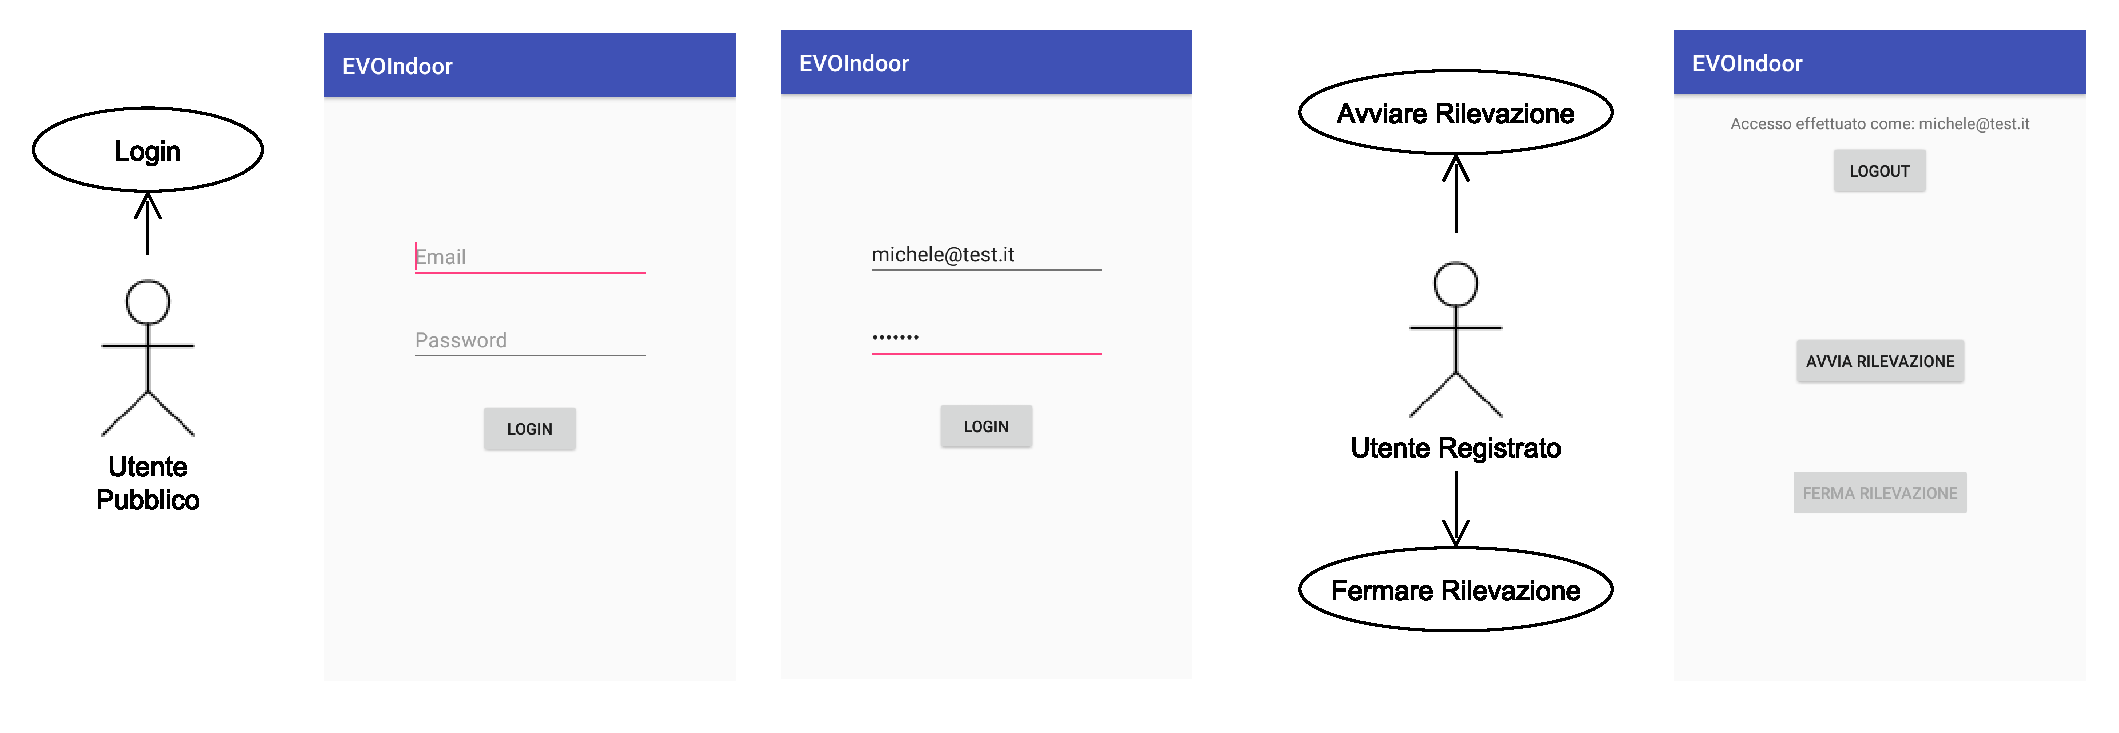
\includegraphics[width=\textwidth]{ucs-android}
	\caption{Casi d'uso applicazione Android}
	\label{fig:ucs-android}
\end{figure}

\begin{figure}[htp]
	\centering
	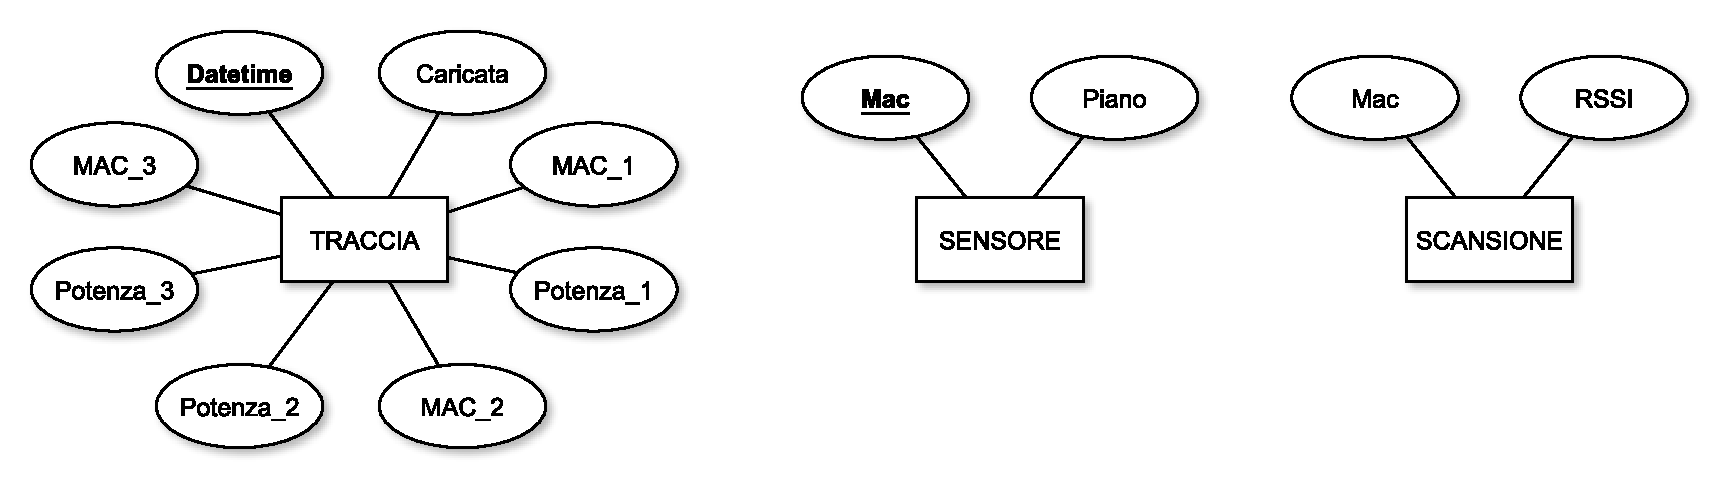
\includegraphics[width=\textwidth]{modello-er-db-android}
	\caption{Modello E-R del database dell'applicazione Android}
	\label{fig:modello-er-db-android}
\end{figure}

Per lo sviluppo delle funzioni del protocollo MQTT si è utilizzata la libreria Eclipse Paho, libreria di riferimento per l’ecosistema MQTT, disponibile open-source in diversi linguaggi.
Al suo avvio la seconda Activity effettua la sottoscrizione al topic in cui è presente la lista dei TAG BLE e, dato che o il localizzatore o il web service hanno pubblicato sullo stesso topic la lista dei TAG BLE disponibili con flag retain, allora si riceve subito la lista dei TAG BLE.

La lista dei TAG BLE serve per poter filtrare durante la scansione dei dispositivi Bluetooth solo quelli che effettivamente risultano essere registrati nella piattaforma, evitando in questo modo di memorizzare l'RSSI di altre periferiche che implementano l’interfaccia Bluetooth LE.

All'avvio della rilevazione, si avvia un service in background composto da due thread \texttt{TracciaUpload} e \texttt{TracciaBuffer}.

Il thread \texttt{TracciaBuffer} finchè la rilevazione è attiva esegue sequenzialmente le seguenti operazioni:
\begin{enumerate}
	
	\item Avvia la scansione dei dispositivi BLE;
	
	\item Attende un secondo;
	
	\item Ferma la scansione dei dispositivi BLE;
	
	\item Filtra le letture dei dispositivi BLE memorizzati, eliminando le letture dei dispositivi che non sono presenti nella lista dei TAG BLE;
	
	\item Esegue la media se sono presenti più valori di RSSI riferiti allo stesso TAG BLE;
	
	\item Aggiunge la traccia al Database, se esistono le letture di almeno 3 TAG BLE distinti, inserendo all'interno della traccia le letture dei 3 TAG BLE con indice RSSI più basso.
	 
\end{enumerate}
La scansione dei dispositivi BLE è realizzata mediante il codice \ref{cod:ble-scan}.

\begin{lstlisting}[language=JavaScript, label=cod:ble-scan, caption=Scansione dei dispositivi BLE]
BluetoothAdapter.startLeScan:
	Callback{
		db.addScansione();
	}
\end{lstlisting}

Il thread \texttt{TracciaUpload} avvia il thread \texttt{TracciaBuffer} e finchè la rilevazione è attiva esegue sequenzialmente le seguenti operazioni:
\begin{enumerate}
	
	\item Attende 2 secondi;
	
	\item Apre una connessione MQTT verso il broker;
	
	\item Invia le tracce memorizzate nel database non ancora inviate;
	
	\item Cancella le tracce inviate dal database;
	
	\item Chiude la connessione MQTT.
	 
\end{enumerate}			% implementazione
	% !TEX encoding = UTF-8
% !TEX TS-program = pdflatex
% !TEX root = ../tesi.tex
% !TEX spellcheck = it-IT

%*************************************************************
\chapter{Risultati sperimentali}
\label{cap:risultati-sperimentali}
%*************************************************************

I risultati ottenuti dal sistema, forniscono delle risposte significative circa la posizione della risorsa. Occorre precisare che la limitata complessità degli algoritmi utilizzati influisce, talvolta negativamente, sulla risposta di localizzazione in alcune particolari situazioni che verranno analizzate a parte.

Di seguito è riassunto l'esperimento effettuato al fine di valutare le performance del sistema.

\section{Deployment del sistema}
La prova è stata effettuata in un reale ambiente aziendale, di circa 300 metri quadrati.

Lo smartphone utilizzato per i test è un Alcatel A3 (TCL 5046Y), terminale Android di fascia bassa, mentre sono stati utilizzati da un minimo di 3 a un massimo di 8 TAG BLE.

Le varie connessioni implementate nell'applicazione Android puntano verso l'indirizzo IP del computer utilizzato per lo sviluppo.
Nel computer utilizzato per lo sviluppo sono stati avviati nell'ordine: il broker mqtt, il localizzatore e il web service.

Si è avviata, accedendo dal browser, la Single Page Application e si è inserita la piantina dell'ambiente indoor che si desidera monitorare. Successivamente, si sono registrati e posizionati i vari TAG BLE all'interno dell'applicazione. Al termine della configurazione si ottiene un risultato come quello in figura \ref{fig:single-page-application}. Successivamente si sono posizionati i TAG BLE, precedentemente registrati nell'ambiente indoor, coerentemente con quanto fatto nell'applicazione.

\begin{figure}[htp]
	\centering
	\includegraphics[height=\textheight/3]{single-page-application}
	\caption{Configurazione dell'ambiente indoor e posizionamento dei TAG BLE nell'interfaccia web}
	\label{fig:single-page-application}
\end{figure}

Si avvia l'applicazione sul dispositivo Android che, dopo aver effettuato l'autenticazione al broker MQTT, riceve e memorizza dal broker la lista dei TAG registrati. Si avvia quindi il tracciamento della risorsa.
A questo punto, l'applicazione Android, invia periodicamente al broker MQTT, per ogni intervallo di tempo, i valori RSSI dei 3 TAG più vicini. Il broker MQTT inoltra i messaggi al localizzatore che si occupa di registrare il messaggio, di effettuare la conversione da RSSI a metri per ogni valore RSSI ricevuto e di ottenere la posizione tramite l'algoritmo di Trilaterazione.

Dalla Single Page Application, avviando la visualizzazione delle risorse, si interroga periodicamente il web service per ottenere l'ultima posizione disponibile di tutte le risorse, visualizzandole nella piantina dell'ambiente indoor come in figura \ref{fig:tracciamento-risorsa}.

\begin{figure}[htp]
	\centering
	\includegraphics[height=\textheight/3]{tracciamento-risorsa}
	\caption{Visualizzazione della risorsa nell'interfaccia web}
	\label{fig:tracciamento-risorsa}
\end{figure}

\section{Valutazione delle performance}
A corredo dell'analisi sperimentale è importante effettuare una stima delle performance del sistema, considerando come indici i parametri fondamentali. Di seguito il sistema è analizzato alla luce dei risultati ottenuti dai test eseguiti a run-time.

\subsection{Accuratezza}
L'accuratezza del sistema dipende da tanti fattori. I test effettuati dimostrano che, con gli algoritmi utilizzati, l'accuratezza della risposta di localizzazione è intorno a 1,5 metri, considerando praticamente sempre di localizzarsi all'interno della stanza giusta. Nei casi limite, ovvero fra una stanza e un'altra, la risposta ``ondeggia'' fra i due TAG BLE di confine.

\subsection{Complessità}
La complessità del sistema risulta tutto sommato bassa, il costo computazionale è limitato ai soli confronti e a pochi calcoli semplici che rendono adatto il sistema anche a terminali più datati.

\subsection{Robustezza}
La robustezza sistema dipende dalla distribuzione dei TAG BLE in funzione dei distrurbi presenti e della distanza, quindi dalla complessità dell'ambiente che si vuole localizzare. Se in un abiente molto disturbato la distribuzione dei TAG BLE è bassa, allora la posizione della risorsa può essere errata a causa di una errata interpretazione dell'indicatore RSSI.

\subsection{Scalabilità}
Il sistema ha come vantaggio un'alta scalabilità che lo rende adatto sia in ambito domestico, che per l'utilizzo in grandi spazi nel quale risulta ancora più performante.

\subsection{Costo}
Come previsto, il costo del sistema è relativamente basso, l'infrastruttura è composta unicamente da TAG BLE e da smartphone, non richiede quindi sistemi dedicati. Altro costo è invece quello di messa in funzione e manutenzione del sistema; sicuramente più elevato, dati i tempi necessari alla costruzione della mappa.			% risultati
	% !TEX encoding = UTF-8
% !TEX TS-program = pdflatex
% !TEX root = ../tesi.tex
% !TEX spellcheck = it-IT

%*************************************************************
\chapter*{Conclusioni}
\addcontentsline{toc}{chapter}{Conclusioni}
\markboth{\MakeUppercase{Conclusioni}}{\MakeUppercase{Conclusioni}}
\label{cap:conclusioni}
%*************************************************************

Lo sviluppo delle comunicazioni wireless, dei dispositivi a basso costo, e in generale il facile accesso alle reti, aprono diverse possibilità di applicazione interessanti per il mercato.

La localizzazione indoor, implementata con TAG BLE, è una soluzione economica e dinamica. L'indice RSSI, come dice il nome, non è la potenza reale ricevuta dall'antenna del nodo ricevente, bensì un indice di questa. L'indice viene calcolato basandosi sul numero di errori di trasmissione rilevati nel pacchetto appena ricevuto, in quanto è giusto aspettarsi un numero di errori più elevato per potenze più basse.

Costruire un modello che caratterizzi al meglio il canale radio dell'ambiente in cui si va a realizzare la localizzazione è estremamente complesso. Sono troppe, infatti, le variabili che possono portare a cambiare significativamente il comportamento del sistema. Tra queste variabili ci sono riflessioni, rifrazioni e multipath del segnale radio assieme ad altri disturbi come oggetti in movimento. Di conseguenza l'indice RSSI non è sicuramente il metodo migliore per effettuare la localizzazione.

Tuttavia, con degli opportuni accorgimenti e con una buona modellazione, si possono ottenere discreti risultati. Dalle verifiche sperimentali è emerso che, per una buona localizzazione non sono necessari algoritmi troppo complessi. L'algoritmo della Trilaterazione, estremamente semplice dal punto di vista logico e computazionale, si è dimostrato accurato e preciso.

Il fatto di utilizzare più TAG BLE in ricezione per compensare eventuali disturbi rappresenta una soluzione molto efficace per aumentare la qualità e l'efficienza della localizzazione, tenuto conto infatti del costo ridotto di un TAG BLE.

Infine, per ottenere dei buoni risultati basandosi sull’indicatore RSSI è sconsigliabile avere scenari molto ampi con pochi TAG BLE.
Nel complesso, nonostante la debolezza intrinseca dell’indice RSSI, si può comunque affermare che il sistema realizzato si comporti bene, ottenendo delle buone localizzazioni con errori di circa 1 metro, in ambiente indoor.

In futuro, il primo miglioramento potrebbe essere un raffinamento nel calcolo della distanza implementando un procedimento di calibratura automatica per quanto riguarda il calcolo dei parametri $A$ e $n$, in modo da velocizzare la fase di caratterizzazione del canale ogni qualvolta si presenti la necessità di operare in un nuovo ambiente. Una procedura di questo genere dovrebbe richiedere all'utente di porre a varie distanze note un dato nodo mobile rispetto ad un nodo riferimento, posizionato nell'ambiente per cui si vogliono calcolare i parametri ambientali. I parametri $A$ e $n$, caratteristici del canale, si possono quindi ricavare provando ad interpolare una funzione di tipo logaritmico utilizzando i valori di RSSI.

Il progetto realizzato ha consentito un approfondimento delle conoscenze dei pattern del linguaggio Java per lo sviluppo di applicazioni Android e per il multithread. Si sono rafforzate, inoltre, le conoscenze riguardo il linguaggio JavaScript, per lo sviluppo di applicazioni sia lato client che lato server.

I framework analizzati e utilizzati durante il periodo di tirocinio erano totalmente sconosciuti, mentre al termine del tirocinio si sono acquisite delle conoscenze basilari riguardo i vari framework. In particolar modo è stata raggiunta una buona padronanza nello sviluppo di applicazioni in Node.js, specialmente nello sviluppo di un'applicazione secondo i pattern tipici, anch'essi sconosciuti prima dell'inizio del tirocinio.

Sempre legato allo sviluppo, sono state acquisite delle competenze riguardo i tools offerti da Android Studio per il debug di applicazioni Android, e Visual Studio Code per il debug di applicazioni lato server, che prima non erano mai stati utilizzati.

Si sono rafforzate, inoltre, le competenze riguardo il linguaggio JavaScript, già conosciuto prima del tirocinio, ma del quale non si conosceva lo standard ES6.

Si sono acquisite delle nozioni riguardo alcuni aspetti del mondo aziendale, in particolar modo si è osservato come un'azienda valuta la possibilità di sviluppare nuove funzionalità stimandone benefici e costi.

Si è osservato, inoltre, come l'esperienza utente e i feedback forniti dai clienti influiscono sulla progettazione di un'interfaccia grafica, costringendo l'utilizzo di strategie per massimizzare le prestazioni al fine di soddisfare le diverse esigenze.			% conclusioni
	
	%**************************************************************
	% Materiale finale
	%**************************************************************
	\backmatter
	% !TEX encoding = UTF-8
% !TEX TS-program = pdflatex
% !TEX root = ../tesi.tex
% !TEX spellcheck = it-IT

%**************************************************************
% Bibliografia
%**************************************************************

\nocite{*}
\printbibliography	% bibliografia	

\end{document}